%\section{introduction}

% Good point, but we don't really need it anywhere:
%
% It would be futile to compare our techniques with one of the
% existing manual regex parsers, as (a) as our literature survey showed,
% their scope is mainly limited to the Java ecosystem and (b) whether
% they would work or not would be randomly based on whether the project
% we select exhibits features their regular expressions were trained for.
% Finally, they are not really automatic

\lstset{
  morekeywords={},
	basicstyle=\ttfamily\scriptsize,
  postbreak=\mbox{\textcolor{blue}{$\hookrightarrow$}\space},
  showspaces=false,
  showstringspaces=false,
  stringstyle=\color{Plum},
	frame=single,
  extendedchars=false,
  texcl=false,
  aboveskip=\baselineskip,
  belowskip=0pt
}

\IEEEPARstart{I}{n}
the past two decades, Continuous Integration (CI) has become a
ubiquitous best practice to streamline the build process of software
projects~\cite{hilton2016usage,beller2017oops,staahl2014modeling}.
Build logs are a textual by-product that these automatic software
builds create.
As a treasure trove of information~\cite{meyer},
build logs contain trace outputs of not only the elementary steps to
``make'' a project---such as retrieving and resolving dependencies and
compiling---but also about ancillary quality assurance steps---such as
testing the software and running automated static analysis
tools~\cite{beller2017oops}.
The
contents and format of build logs can vary highly depending on which tools
are involved in the build process, how they are
configured, and as projects and build tools evolve over
time~\cite{staahl2014modeling}.
Typically, though, they are at least a semi-structured and
somewhat stable journal of the commands executed during the build and
their results.

When a build or one of its steps fails, developers typically scavenge
the logs for information related to the source of the error.
This
manual activity is tedious and prone to
errors~\cite{santolucito2018statically}.
As a single build log can be
over 50 megabytes large~\cite{beller2017oops}, finding the small chunk
of information linked to the actual error, is akin to
searching for a needle in a haystack.
The large number of unrelated, but ambiguous
warnings which many build
logs regularly contain further compounds this problem.
In addition to helping
understand and fix build failures, the information richness of build
logs enables a plethora of other applications: with the help of build
logs, we can better understand and categorize CI failures and compile
errors~\cite{islam2017insights,seo2014programmers}, differentiate
testing practices~\cite{orellana2017differences,vassallo2017a-tale},
train classifiers to do ``predictive CI'' on the build or test outcome
and
duration~\cite{ni2017cost,bisong2017built,haghighatkhah2018test,
machalica2019predictive},
or investigate the role of automated static analysis tools (ASATs)
in CI
builds~\cite{zampetti2017open}.

However, manual analysis of build logs does not
scale to the number of build logs and amount of information that such
sophisticated applications require.
Moreover, being able to
automatically extract relevant pieces of information from build logs
can help
developers debug a broken build more quickly without having to browse
the entire build log.

\begin{figure*}[htb]
	\centering
	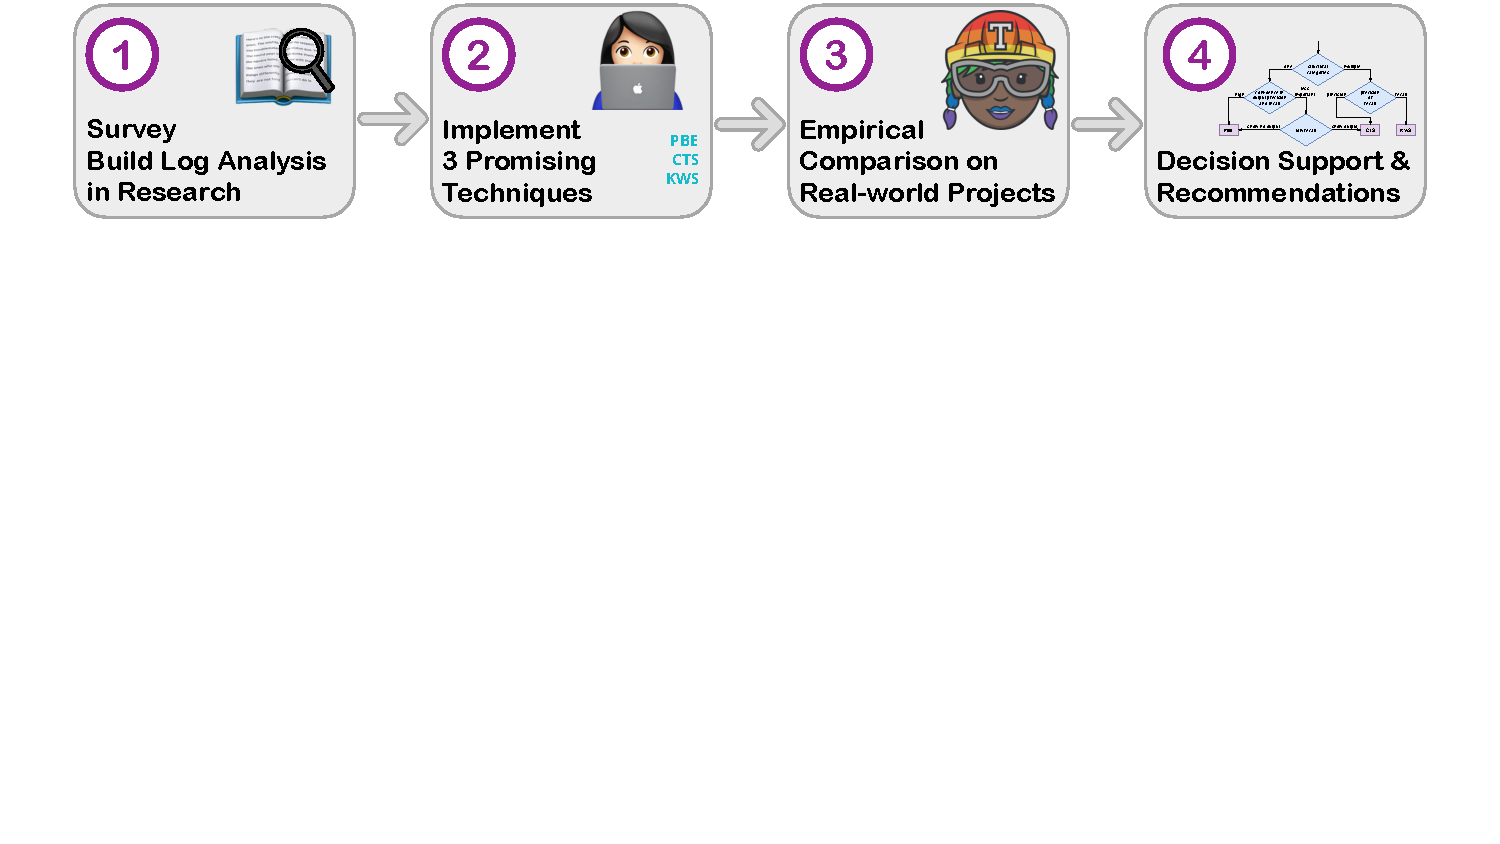
\includegraphics[width=\textwidth, trim={1.2cm 10.5cm 1.2cm 0cm},
	clip]{img/overview.pdf}
	\caption{Research design.}
	\label{fig:overview}
\end{figure*}

Retrospectively analyzing the build logs is not the only solution to
the problem---an alternate would be to integrate live plugins into the
build process
 such as the JUnit
plugin for Jenkins~\cite{jenkins2020junit-plugin} or
Deflaker by Bell et al.~\cite{bell2018deflaker}.

Their advantage is that they can precisely report the information which
is required.
However, such plugins are not available for all build tools, they are
non-trivial to implement one-off solutions, and they
do not enable the analysis of historical builds.
When using such a plugin, one has to decide
beforehand which information should be reported, whereas
build log analysis enables us to leverage all information
present in the build logs.
Moreover, build log analysis is the more general solution.
While they serve an important niche, custom plugins do not make build
log analysis redundant.

Despite its central role in helping developers and in enabling
novel, onward processing applications,
the process of how to
automatically
analyze build logs has thus far not been systematically
overviewed as a research topic, bringing us to the first
research question:
\begin{simplebox}[minipage boxed title*=-5cm]{\textbf{Research Question
1}}
What is the state-of-research to analyze build logs?
\end{simplebox}

To answer this question, we start the investigation in this
paper---pictured in
\Cref{fig:overview}---with an
extensive literature survey (step \circlenum{1}).
The survey identifies various strategies to
analyze build logs, among which are developing
custom parsers, using regular expressions, doing manual inspections,
searching for keywords, or performing natural language processing.

However, it also identifies that there is currently no guidance on when
to use which of these
approaches.
Unfortunately, our survey also shows that
less than half of the 61 works which rely on build log analysis
describe it in sufficient detail and that
the few available implementations are all based on either a custom parser
or regular expressions.
These two approaches are problematic, as their creation
and maintenance is manual and expensive, does not generalize across build
logs from different build tools, and is prone to errors,
as the experience of
TravisTorrent has
shown~\cite{beller2017travistorrent,travistorrentquestions}.
In fact, some even ``strongly discourage'' the creation of such
parsers~\cite{urli2018design}.
In summary, the outcome of our literature survey shows the need for a new
generation of automated techniques to analyze build logs, which are
openly available and documented in detail, together with
guidance on when to use which technique.

To fill this gap, we created three novel, prototypical
implementations to
automatically analyze build logs (step \circlenum{2}).
The ideas behind the implementations are based on promising approaches
adopted from other research fields and existing build log analysis
techniques by retrieving a substring (chunk) from the build log:
\begin{itemize}
	\item \emph{Program Synthesis by Example (PBE)}, a technique
	able to
	automatically synthesize regular expressions,
	\item a technique based on information
	retrieval, using \emph{Common Text Similarity (CTS)},
	\item inspired by the manual ad hoc search for key parts in the
	log, a
	technique employing \emph{Keyword Search (KWS)}.
\end{itemize}

These three approaches have
different strengths and weaknesses.
As a consequence,
in the second research question we ask:

\begin{simplebox}[minipage boxed title*=-5cm]{\textbf{Research Question
2}}
How do build log analysis techniques compare?
\end{simplebox}

To answer this question
we conduct an empirical study assessing the performance
of these chunk retrieval techniques in
real-world projects under a variety of conditions (step \circlenum{3}).
The study is based on the \emph{LogChunks} data
set~\cite{brandt2020logchunks}, which encompasses 797 build logs from
80 popular open-source projects and a broad range of different
build tools and programming languages.
Our results show that all of the three techniques
clearly surpass a random baseline, but have different strengths and
weaknesses.
There is no technique that in general outperforms
the others.
PBE has the best average precision of 95\%, while KWS has the highest
recall with 70\% on average.
However, CTS shows the best F$_{1}$-score
of 51\%.


Due to this ambiguity, we develop a set of guidelines
on how to choose the most suitable build log analysis
technique for the task at hand (step \circlenum{4}).
We recommend PBE for use cases where the desired information is always
represented in the same structural way and high confidence in
precision and recall of the chunk retrieval is required.
The results PBE produces are suited for automatic onward processing.
CTS is
well-suited when the representation of the desired information varies
slightly and the output of the chunk retrieval is further processed by
a human.
In cases where the textual representation of the desired
information in the log is unpredictable or varies greatly, KWS seems
to be the best choice.
However, its low precision---it extracts a
context of multiple lines around a found keyword---makes it generally
unsuited for automatic onward processing.
Instead, KWS requires a human
to further inspect and interpret the output chunk.
A hybrid solution combining the three techniques might be the best
all-round solution.
Finally, we give a roadmap to guide future research in the field
of build log analysis.

In short, this article contributes
\begin{itemize}
\item the first systematic survey of the emerging field of build log
analysis.
\item three prototypical open-sourced implementations of
promising chunk retrieval techniques.
\item a large empirical study comparing the three techniques.
\item systematic guidelines on when to use which technique.
\item a detailed research map to inspire future contributions to the
field.
\item a documented replication package~\cite{brandt2020chunk-replication}.
\end{itemize}

\begin{figure}[tb]
	\centering
	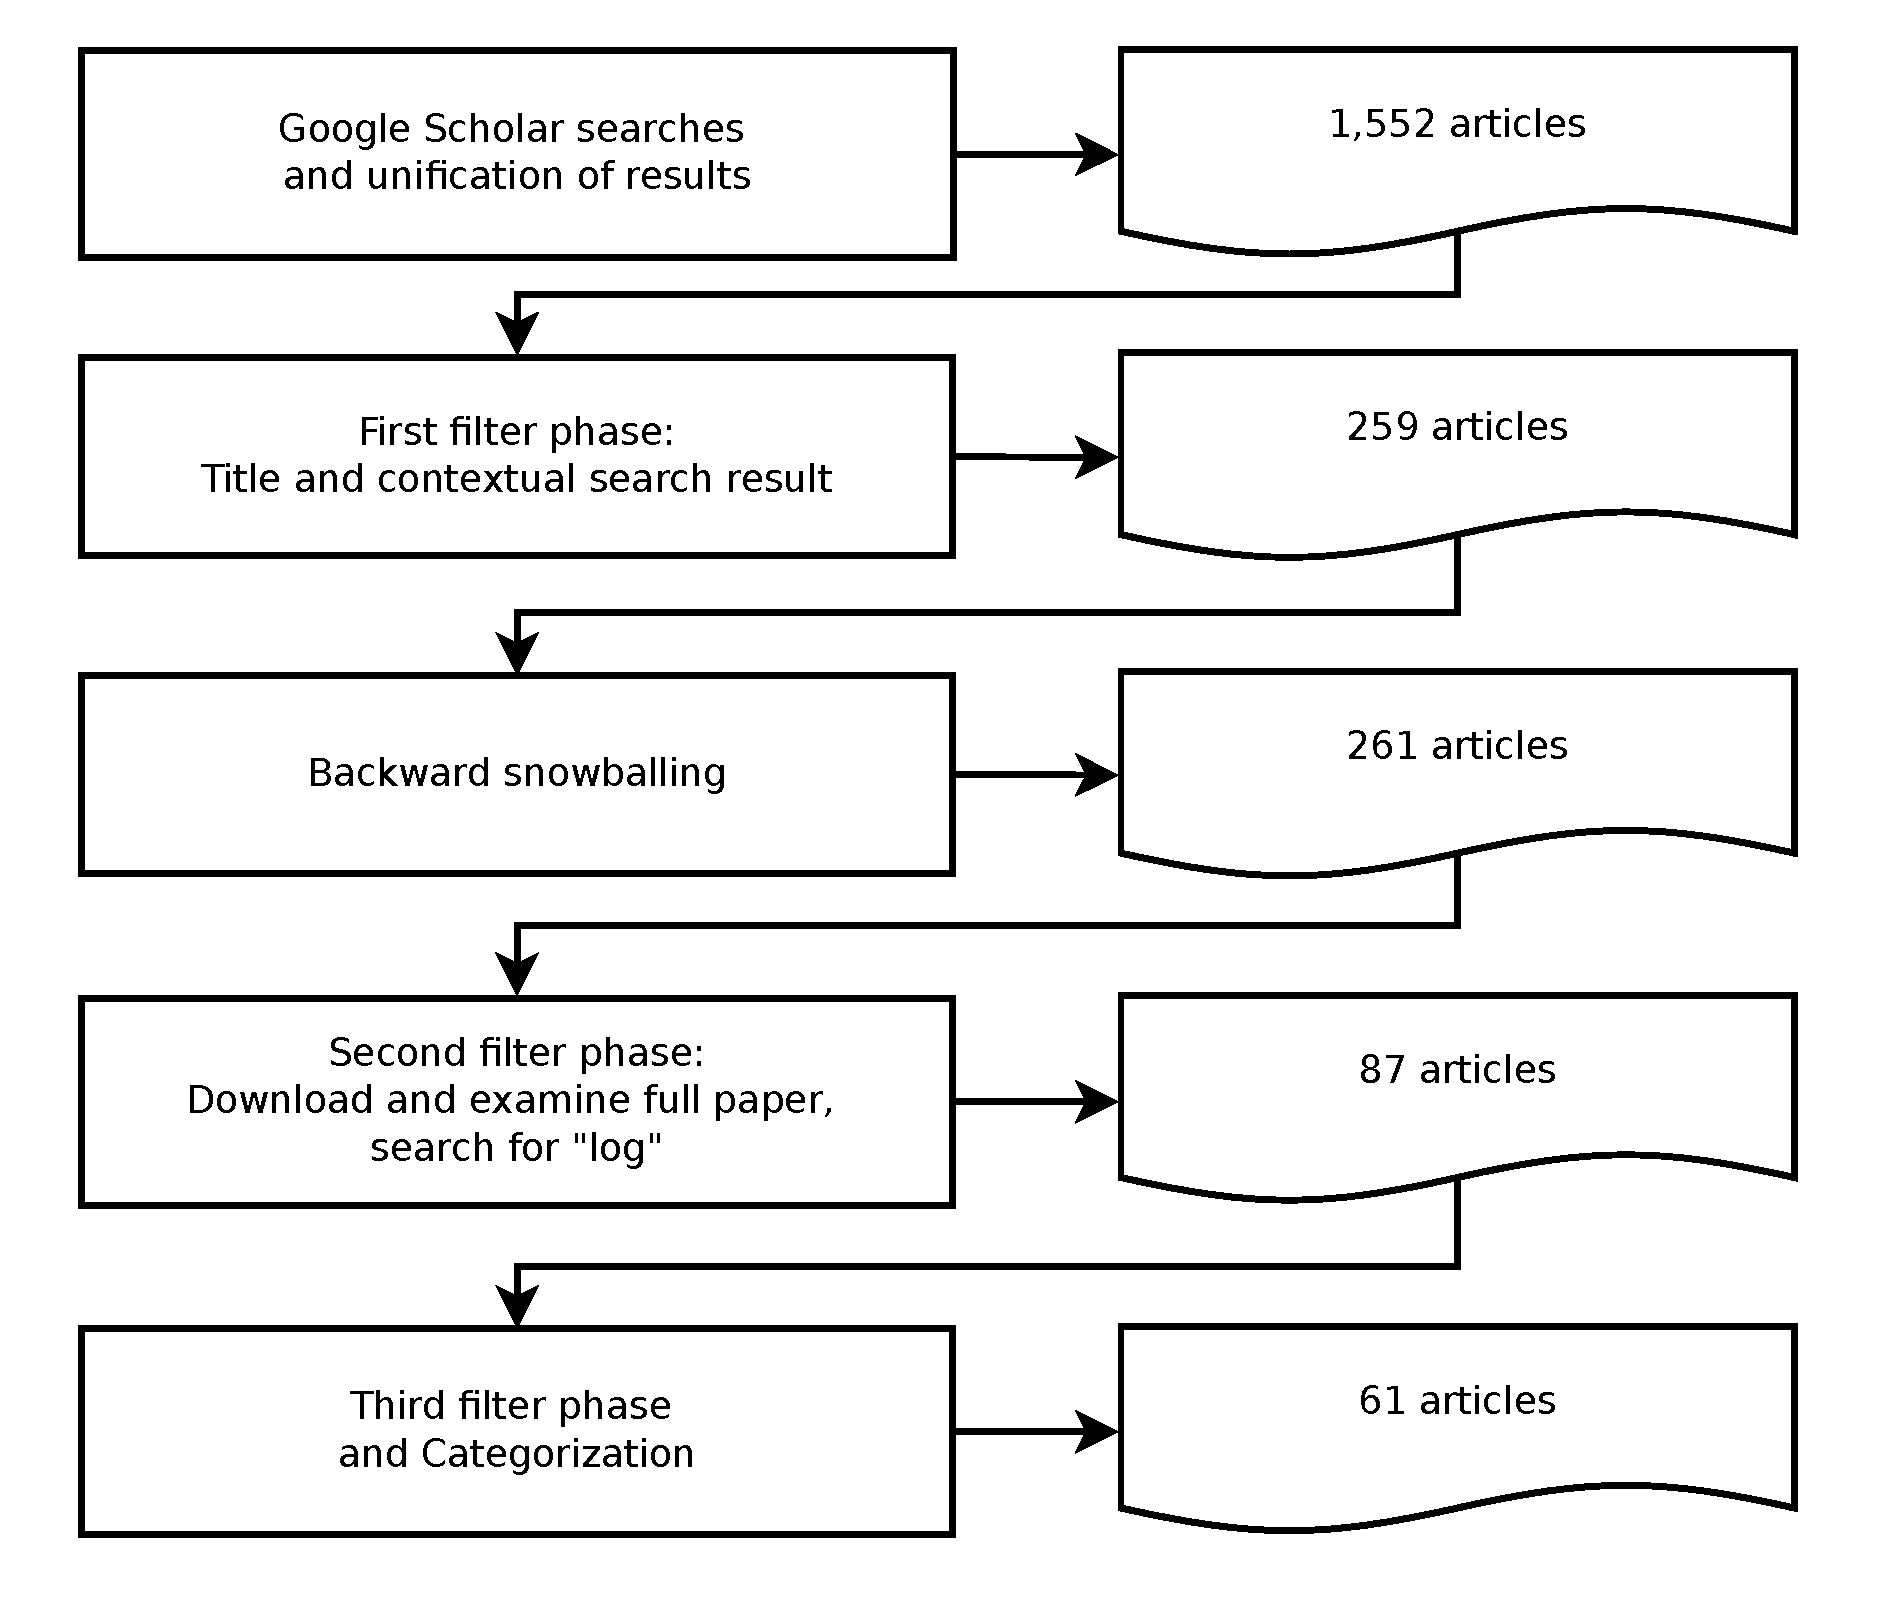
\includegraphics[width=\columnwidth, clip]{img/lit_survey.pdf}
	\caption{Literature selection (following Petersen et
	al.~\cite{petersen2015guidelines}).}
	\label{fig:lit-survey}
\end{figure}

\section{Systematic Literature Mapping Survey}
\label{sec:survey}
% tense: past

In this section, we report on the state-of-research in the emerging
field of build log analysis by means of a systematic mapping study.
We start with a differentiation of build log analysis
from the older field of
system log analysis.
% ref to fig 2 so it can be here and above fig 3
Then, we describe the methodology (\Cref{fig:lit-survey})
and results of our systematic mapping
survey following the
guidelines by Petersen et
al.~\cite{petersen2008systematic,petersen2015guidelines}.
% We close by summarizing how build logs are commonly
% analyzed in literature and discuss the implications of these findings.

\lstset{
  morekeywords={INFO, WARN, 2008, 11, 09},
  alsoletter=-20819,
  keywordstyle=\bfseries\color{Plum},
  escapeinside=**
}
\begin{figure}[b]
  \centering
  \lstinputlisting[breaklines=true]{listings/syslog.txt}
  \caption{System log excerpt (adapted from He et
  al.~\cite{he2017towards}).}
  \label{lst:system-log}
\end{figure}

\subsection{Distinction from System Log Analysis}
\label{sec:system-log-analysis}
% tense: present

A field related to build log analysis is the analysis of system logs.
These system logs are produced during the runtime of a system, while
build logs are produced during the runtime of the build of the system.
In terms of the contents of the logs, the main difference is that system
logs are fundamentally structured
through events.
Each line in a log file represents one event with a
set of fields: timestamp, verbosity level, and raw message
content~\cite{he2017towards}.
\Cref{lst:system-log} depicts two
exemplary lines from such a system log.

When analyzing system log files, the first goal is generally to
separate the constant and variable parts within a log
message~\cite{nagappan2010abstracting,he2017towards}.
Next, the log
messages are clustered into log events, unifying messages with
identical constant parts and varying parameters.
The output is an
ordered list of timed events and their corresponding parameter
values~\cite{he2016evaluation}.
This structured log can serve as
input to various machine learning and data mining processes.
Apart
from a large body of research on system logs, an equally mature amount
of commercial-grade and
open source tooling exists to analyze system logs---such as, for
example, Elasticsearch, Logstash and Kiabana (the so-called ELK
stack)~\cite{sanjappa2017analysis,bajer2017building}.

Some of the techniques developed to parse system logs can operate
on build logs as well, such as approaches to retrieve the
values of variable parts in a log message, e.g.\, by using regular
expressions~\cite{nagappan2010abstracting,xu2009detecting}.
% This is the easiest example matching here
% amar et al are not in our literature survey
However, the number of
system logs generated mandates that scalability and efficiency play a
much more important role than for build logs.
In addition, almost all of the techniques developed to analyze system logs
leverage their inherent event structure.
Build logs generally lack this
structure and thus require different bespoke approaches.
% if included: this explanation is not understandable.
% It needs to better embedded in the surrounding text
% One example is comparing execution traces to reference
% traces of intended behavior to detect anomalies.
% Amar et
% al.~\cite{amar2019mining} employed a similar approach to detect
% relevant lines in build logs.
% In this article, we focus on extracting a single specified information
% from the build log as a whole with chunk retrieval techniques.
% Chunk
% retrieval techniques are used as a part of log parsing

\subsection{Literature Selection}
\label{sec:litsel}
% tense: past

The first step in a systematic literature survey is to
establish which works one wants to cover and how to find
them~\cite{kitchenham2009systematic}.
Since the field of build log analysis is relatively young, we
surveyed as broad a population of scientific material as possible.
We did not limit the sources to specific Software Engineering
venues~\cite{petersen2015guidelines}, but included all sources
monitored by Google Scholar, including Bachelor's theses, Master's
theses, and academic slide decks.
We use Google Scholar as opposed to Scopus or
other databases because it is the search engine for scholarly material
with
the broadest and most current index, including preprints.

\Cref{fig:lit-survey} gives an overview of the literature selection
process.
An initial Google Scholar search for ``build log''
returned more than 2.2 million results on the 15th of March 2020, many
of which stem
from unrelated fields such as construction or wood working.
We refined the search criteria to exclude such obvious
non-related fields and to exclude works on system
logs (see \Cref{sec:system-log-analysis}).
This left us with 1,552 search results.
% Our replication package documents the full search
% queries~\cite{brandt2020chunk-replication}.
To make handling so many search results feasible, we employed a
three-pass filtering strategy:

First, we filtered works based on (a) their title and (b) the
contextual information Google Scholar displayed on its search results
page.
We included works at large that seemed to bear a resemblance to software
engineering and building software.
Following Kitchenham's protocol~\cite{kitchenham2009systematic},
we excluded
works written in a language unintelligible to the authors
(i.e., not English or German), which disregarded fewer than 1\% of search
hits.
% 'four' not clear and it gets lost that there are multiple search queries
% therefore I'll cut this part completely:
% We then unified
% the results of the four search queries based on the link as the
% identifying element, removing 60 works that appeared in more than
% one search query.
We removed duplicates based on the title and were
left with 256 works (16\% of the original search results).

With these 256 remaining works, we followed a backward snowball
sampling for related work.
If a work referenced a new work in the context
of build log analysis, we added the new one to the literature set.
This added five works (eight before
duplicate elimination), leading to a total of 261
works.

Second, we performed a finer filter phase by (1) reading abstracts,
and (2) downloading the
full text of the works and searching it
for the occurrence of the term ``log.''
If a work showed traces of
working with build logs, we passed it onto the final filter phase.
In total, we
were left with 87 works after the second filtering phase.

Third, since we had been careful to include rather than exclude borderline
works, a deeper evaluation excluded another 15 works from the 87
works left after the second filter phase.
Multiple works were extensions of others.
Of these, we only considered the earliest work which reported on
the analyzing of build logs.
This excluded another 11 works.
In sum, we included and classified 61 works in detail.

\subsection{Literature Classification}
Having trimmed down the set of works by 95\%, we investigated the
remaining ones in-depth.
Our aim was to characterize how researchers work with build logs.

Specifically, we were interested in
\begin{itemize}
  \item what information the researchers retrieve from build logs and
  what they use this information for (\textbf{RQ1.1}),
  \item which techniques they employ to process the build logs,
  in how much detail the techniques are described,
	and whether their implemented tools are published
  (\textbf{RQ1.2}),
  \item which kinds of build logs the researchers analyze
	and the origin of these logs (\textbf{RQ1.3}).
\end{itemize}

This lead us to the following research questions:
\begin{simplebox}[attach boxed title to top center={yshift=-6mm}]
{\textbf{RQ1:} What is the state-of-research to analyze build logs?}
\begin{itemize}[leftmargin=1cm]
  \item[\textbf{RQ1.1:}] What information is targeted in build logs?
  \item[\textbf{RQ1.2:}] Which analysis techniques exist?
  \item[\textbf{RQ1.3:}] Which kinds of build logs are subject to
  analysis?
\end{itemize}
\end{simplebox}

To support the data extraction we created a template which we filled out
for each of the 61 works.
The template contained questions to answer RQ 1.1 through RQ 1.3,
for example ``Is the technique explained in detail?'' and
``What is the source of the build logs?''
As recommended by Petersen et
al.~\cite{petersen2015guidelines}, we started the mapping survey with a
pilot:
both authors extracted data from the same five works and held a
consensus meeting to unify their understanding
of the data extraction template.
We divided the remaining 56 works evenly between the two authors
and inspected each work as closely as necessary to fill out the
template
with confidence,
starting from occurrences of ``log'' or ``build'' within the full
text of the work.

For questions that did not require a boolean answer, we allowed assigning
multiple tags or categories as the first part (``preparation phase'')
of a virtual open card sorting~\cite{zimmermann2016card}.
An example of this is the question ``What is the source of the build
log?,''
where we assigned tags such as ``Travis CI,''
``Industrial,'' ``Google,'' or
``Self-built.''
Once we had classified all works, we went into the second phase of
card sorting
(``execution phase''), in which we grouped tags
together and found synonyms.
% the following adds to the example but is maybe unneeded / too much
For instance, in the case of the build log source we grouped
``Travis'' and ``Travis CI'' together and assigned ``Industrial'' to
all works that used build logs from a company.
The replication package contains the data extraction template and all
results of this step~\cite{brandt2020chunk-replication}.


\subsection{Results}
% tense: past
\addtolength{\tabcolsep}{-5pt}
\label{sec:litsurresults}

In this section, we first give a general overview over our paper
population.
We then present the results of the analysis phase along RQs 1.1 through
1.3.

\subsubsection{Descriptive Study Statistics}
\begin{figure}[tbp]
		\centering
		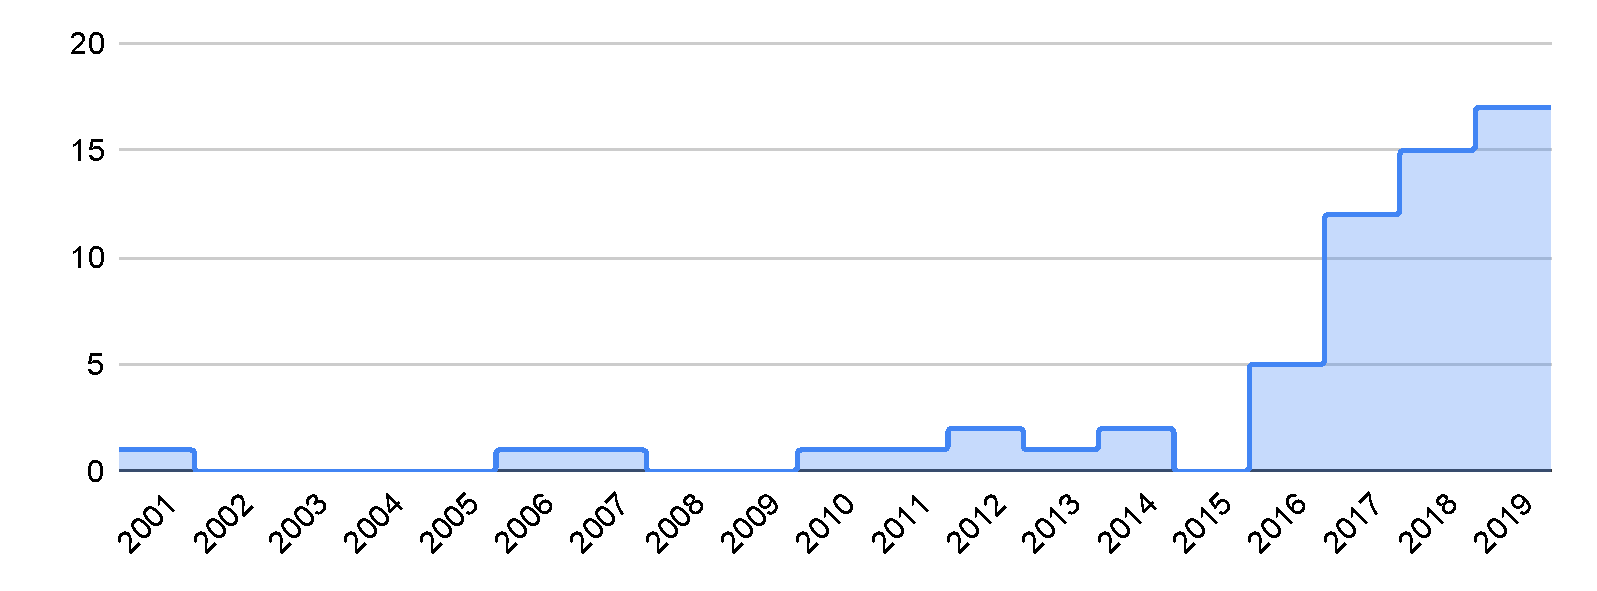
\includegraphics[width=\columnwidth,
		clip]{img/lit-sur/years.pdf}
		\caption{Number of works analyzing build logs per year.}
		\label{fig:lit-years}
\end{figure}

After the third filtering phase, we finally included 61 works in the
literature survey.
The majority of these are scientific articles (81\%), of which all but
three have been peer-reviewed and published (94\%).
The remaining works are theses (14\%), two books, and one slide deck.

\Cref{fig:lit-years} depicts the year of appearance of these
works.
Although we applied no filtering by year in our initial search queries
(see \Cref{sec:litsel}), the earliest work in our literature corpus
stems only from 2001.
There are various scattered works in the years between then and 2016,
when the field of build log analysis started to grow rapidly.


\subsubsection{What information is targeted in build logs? (RQ 1.1)}
\label{sec:rq11}
\begin{figure}
\centering
\begin{subfigure}[t]{\columnwidth}
		\centering
		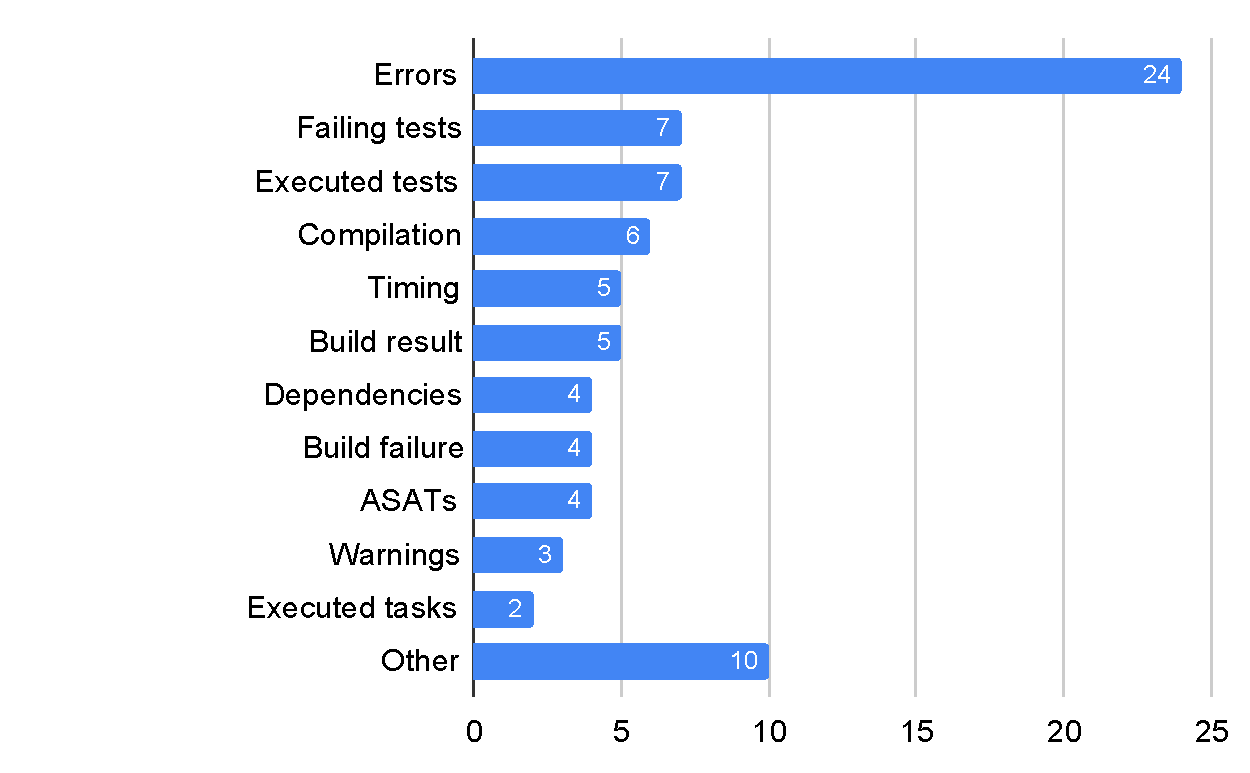
\includegraphics[width=\columnwidth,
		clip]{img/lit-sur/info_target.pdf}
		\caption{Information targeted in build log analysis.}
		\label{fig:litsur:info_target}

\end{subfigure}\hspace{\fill}
\begin{subfigure}[t]{\columnwidth}
		\centering
				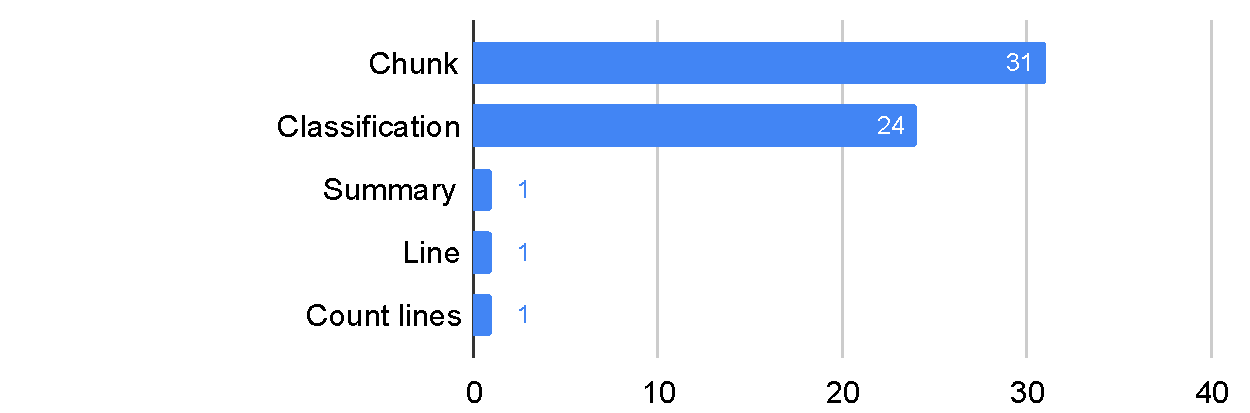
\includegraphics[width=\columnwidth,
				clip]{img/lit-sur/kind.pdf}
		\caption{Class of information analyzed.}
		\label{fig:litsur:kind}

\end{subfigure}
\begin{subfigure}[t]{\columnwidth}
		\centering
				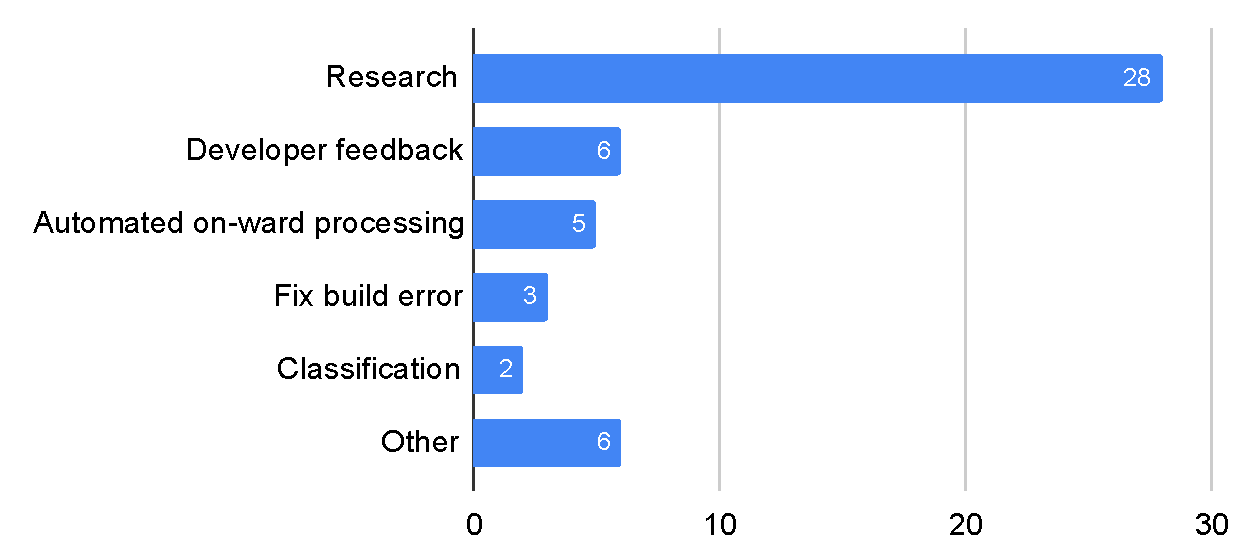
\includegraphics[width=\columnwidth,
				clip]{img/lit-sur/use.pdf}
		\caption{Purpose of build log analysis.}
		\label{fig:litsur:use}

\end{subfigure}

\caption{Multi-label categorization of the 61 relevant works.}
\label{fig:litsur_r}
\end{figure}

In this section, we describe what sort of information the works in
our survey usually retrieve from build logs.
\Cref{fig:litsur_r} depicts these results.

\Cref{fig:litsur:info_target} gives an overview over the frequency of
the targeted information.
The precise information targeted in the build logs varied from work
to work, with a relatively long tail.
Most prominent was the search for errors (39\%), followed by extracting
the executed or the failing
tests (both 11\%).
There were also numerous works which targeted more specialized
information, such as the environments used during the
build~\cite{zolfagharinia2017not}, packages
installed~\cite{selberg2012use}, or hints to source files which
relate to build failures~\cite{ren2018automated}.

\Cref{fig:litsur:kind} depicts that there are two widely used ways to
extract information from build logs: either chunks (53\%) or
classifications (41\%).
Uses for chunks were extracting compilation errors,
test failures, or the duration of build
tasks~\cite{clemencic2014new,zhang2016android}.
Examples for
classifications were distinguishing failures caused by developers from
failures caused by infrastructure errors~\cite{lindqvist2019detection}
or determining whether projects use automated static analysis
tools~\cite{kavaler2019tool}.
Categorization is the more abstract representation, chunks
contain more information and could be turned into a categorization.

\Cref{fig:litsur:use} shows the aim for the
investigated works to analyze build logs, and the result also explains
the prevalence of classification in \Cref{fig:litsur:kind}.
The majority of works (46\%) used the outcome of their build log
analysis to drive further research---and it is science's aim to
classify and abstract.
Seo et al.~\cite{seo2014programmers}, for example,
categorized the types of compile errors encountered at
Google.
Other works (10\%) used the gained insights to give feedback to
developers.
For 8\% of the works was the retrieved information the input
to a next automatic onward processing step:
works chose
tests that should be part of a reduced, but still effective test
suite~\cite{shi2018evaluating} or filled     a data structure with
build information, an information source for further tools aiming
to fix a failing build~\cite{vassallo2018un-break}.

\subsubsection{Which analysis techniques exist? (RQ 1.2)}
\begin{table*}[tbhp]
\tinyish
\centering
\caption{Overview of build log analysis techniques.}
\begin{tabularx}{\textwidth}{@{}lXl@{}}

\toprule
Name			     & Sources	& Frequency	  \\
\midrule

\raisebox{0.8mm}{Parser} &
\raisebox{0.8mm}{
\cite{vassallo2018un-break,zhang2016android,seo2014programmers,hassan2019tackling,hassan2017automatic,chromy2007integration,mesbah2019deepdelta,wen2018blimp,kwon2018prioritizing,adams2007design,rahman2018impact,brandyberry2006continuous,tomassi2019bugswarm,ren2018automated,vassallo2019automated,cavalcanti2019impact,sippola2013qt,felipe2012towards,shi2018evaluating,urli2018design,selberg2012use}
} &

\includegraphics[width=0.55\columnwidth]{img/lit-sur/techniques-no-guidelines-cropped_21.pdf}
\\

\raisebox{0.8mm}{Regular expression} &
\raisebox{0.8mm}{
\cite{beller2017oops,hassan2017change,macho2018automatically,vassallo2017a-tale,lou2019history,hassan2017automatic,rott2019empirische,zampetti2019study,zhao2018comparing,rausch2017empirical,ghaleb2019studying,zampetti2017open,zhang2019large,kavaler2019tool,morris2010experience}
} &

\includegraphics[width=0.55\columnwidth]{img/lit-sur/techniques-no-guidelines-cropped_15.pdf}
\\

\raisebox{0.8mm}{Manual inspection} &
\raisebox{0.8mm}{
\cite{sulir2016quantitative,hassan2017automatic,bouabana2019theory,barinov2017applying,silva2018build,ghaleb2019empirical,marcozzi2019systematic,hukkanen2015adopting,rausch2017empirical,hassan2017mining,zolfagharinia2017not,cassee2019impact}
} &

\includegraphics[width=0.55\columnwidth]{img/lit-sur/techniques-no-guidelines-cropped_12.pdf}
\\

\raisebox{0.8mm}{Machine Learning} &
\raisebox{0.8mm}{
\cite{hassan2017change,lou2019history,lindqvist2019detection,ren2018automated,schulz2017active}
} &

\includegraphics[width=0.55\columnwidth]{img/lit-sur/techniques-no-guidelines-cropped_5.pdf}
\\

\raisebox{0.8mm}{Natural Language Processing}	&
\raisebox{0.8mm}{
\cite{hassan2017change,lou2019history,schulz2017active}
} &

\includegraphics[width=0.55\columnwidth]{img/lit-sur/techniques-no-guidelines-cropped_3.pdf}
\\

\raisebox{0.8mm}{Information Retrieval} &
\raisebox{0.8mm}{
\cite{hassan2017change,lindqvist2019detection,ren2018automated}
} &

\includegraphics[width=0.55\columnwidth]{img/lit-sur/techniques-no-guidelines-cropped_3.pdf}
\\

\raisebox{0.8mm}{Analysis} &
\raisebox{0.8mm}{
\cite{sulir2016quantitative,haghighatkhah2018test,durieux2019critical}
} &

\includegraphics[width=0.55\columnwidth]{img/lit-sur/techniques-no-guidelines-cropped_3.pdf}
\\

\raisebox{0.8mm}{Keyword Search} &
\raisebox{0.8mm}{
\cite{brandyberry2006continuous,zhang2019large,kavaler2019tool}
} &

\includegraphics[width=0.55\columnwidth]{img/lit-sur/techniques-no-guidelines-cropped_3.pdf}
\\

\raisebox{0.8mm}{Scan} &
\raisebox{0.8mm}{
\cite{clemencic2014new,hibbard2001visualization}
} &

\includegraphics[width=0.55\columnwidth]{img/lit-sur/techniques-no-guidelines-cropped_2.pdf}
\\

\raisebox{0.8mm}{Other} &
\raisebox{0.8mm}{
\cite{zhang2016android,hassan2017change,lou2019history,silva2018build,ren2018automated,schulz2017active}
} &

\includegraphics[width=0.55\columnwidth]{img/lit-sur/techniques-no-guidelines-cropped_10.pdf}
\\

\raisebox{0.8mm}{None identified} &
\raisebox{0.8mm}{
\cite{macho2017preventing,felipe2012towards,orellana2017differences,madeyski2017continuous,zhao2017impact,santolucito2018statically,makihara2018multi,mcintosh2012evolution,gallaba2018noise,matthies2016scrumlint}
} &
\\

\specialrule{\heavyrulewidth}{0pt}{2pt}

\end{tabularx}
\label{tab:litsur:techniques}
\end{table*}
\addtolength{\tabcolsep}{5pt}

Of the 61 works we inspected, 43 mentioned how they analyzed
build logs.
However, only 16 of these described their technique in detail.
We summarize the techniques that the works
described for analyzing build logs in \Cref{tab:litsur:techniques}.

The most mentioned technique (34\%) was using a parser.
In this tag, we also
included
rather imprecise statements like ``we parse the build
logs''~\cite{rahman2018impact}.
For such imprecise statements it was often not clear if they described
a complex parser (including a tokenizer, lexer, etc.) or referred to a
simpler parsing tool based on regular expressions.
If we saw evidence for the latter, we assigned the tag
``Regular Expression'' instead of the tag ``Parser.''
25\% of the works described the use of regular expressions and 20\%
inspected the logs manually.
For example,
Seo et al.~\cite{seo2014programmers} developed a custom
parser to classify error messages, while Vassallo et
al.~\cite{vassallo2017a-tale} analyzed build logs with regular
expressions.
Ghaleb et al.~\cite{ghaleb2019studying} used a compound approach.
They started with a manual categorization of build logs and selected
search strings that identify the target category.
Based on the search strings they created a script that automatically
classifies the remaining logs.
Another 8\% of the investigated works
employed machine learning such as natural language
processing or information retrieval techniques.
The rather general tags ``analysis'' and ``scan'' in
\Cref{tab:litsur:techniques}, stem---similar to the imprecise
statements about parsing---from the
words authors used to describe their techniques.
%such as
%``automatically analyzed [the build logs]''.


Only 25\% of the works claimed their implementation is available.
Moreover, we
saw some reuse of the few available build log analysis tools.
Five works employed the tools used to create
\emph{TravisTorrent}~\cite{beller2017oops,
orellana2017differences,zhao2018comparing} or
an updated version of them~\cite{rott2019empirische,
shi2018evaluating}, two used the
\emph{Maven Log Analyzer}~\cite{macho2018automatically,gallaba2018noise},
and
another two
\emph{MAKAO}~\cite{wen2018blimp,adams2007design}.

\subsubsection{Which kinds of build logs are subject to
  analysis? (RQ 1.3)}
As the structure of build logs can change greatly depending on which
build tools output to it~\cite{staahl2014modeling},
we were interested in which build tools are
investigated in the literature.
\Cref{fig:litsur:log_producer} shows the distribution of
build tools whose logs were analyzed by the works in our survey.
Of the works, 30\% analyzed
Maven~\cite{maven2019website},
16\% analyzed Gradle~\cite{gradle2020website},
and 10\% analyzed Ant build logs~\cite{ant2020website}.

A large fraction of the works analyze build logs
from a small number of build tools.
In most cases, this is because the format of build logs
changes and
therefore ``parsers must be specialized to each build and test
framework''~\cite{tomassi2019bugswarm}.
Sometimes, aspects separate from the build log analysis motivate
the limitation to a specific build tool.
For example, Shi et al.
focussed on Maven
build logs because they also chose the PIT tool~\cite{coles2016pit}
to calculate coverage
and mutation score~\cite{shi2018evaluating}.
PIT is only available as a Maven plugin.
Only 7\% of the proposed techniques claimed to be
build tool-agnostic, while
several described that they cover multiple build tools.
The majority of works (42\%) analyzed logs produced by a build tool
that no second work investigated.

In 38\% of cases, the works collected build logs from Travis
CI~\cite{travisci2019webpage};
18\% of the works analyzed logs from TravisTorrent; and 8\% included
build logs from industrial projects.
The number of logs analyzed varied greatly between the works
and we were not always able to
extract it confidently.
23 of the works analyzed more than a thousand build logs, while one
investigated up to 122 million logs.
Of the surveyed works, 31\% claim to have published their data to
enable further research.
However, we found no clear reuse of build log data sets with the
exception of TravisTorrent~\cite{beller2017travistorrent}, which
Vassallo et al.~\cite{vassallo2017a-tale},
Ghaleb et al.~\cite{ghaleb2019studying},
and several others have studied~\cite{hassan2017change,
hassan2019tackling,hassan2017automatic,orellana2017differences,
haghighatkhah2018test,madeyski2017continuous,ghaleb2019empirical,
santolucito2018statically,gallaba2018noise,shi2018evaluating}.

\begin{figure}[tbp]
		\centering
		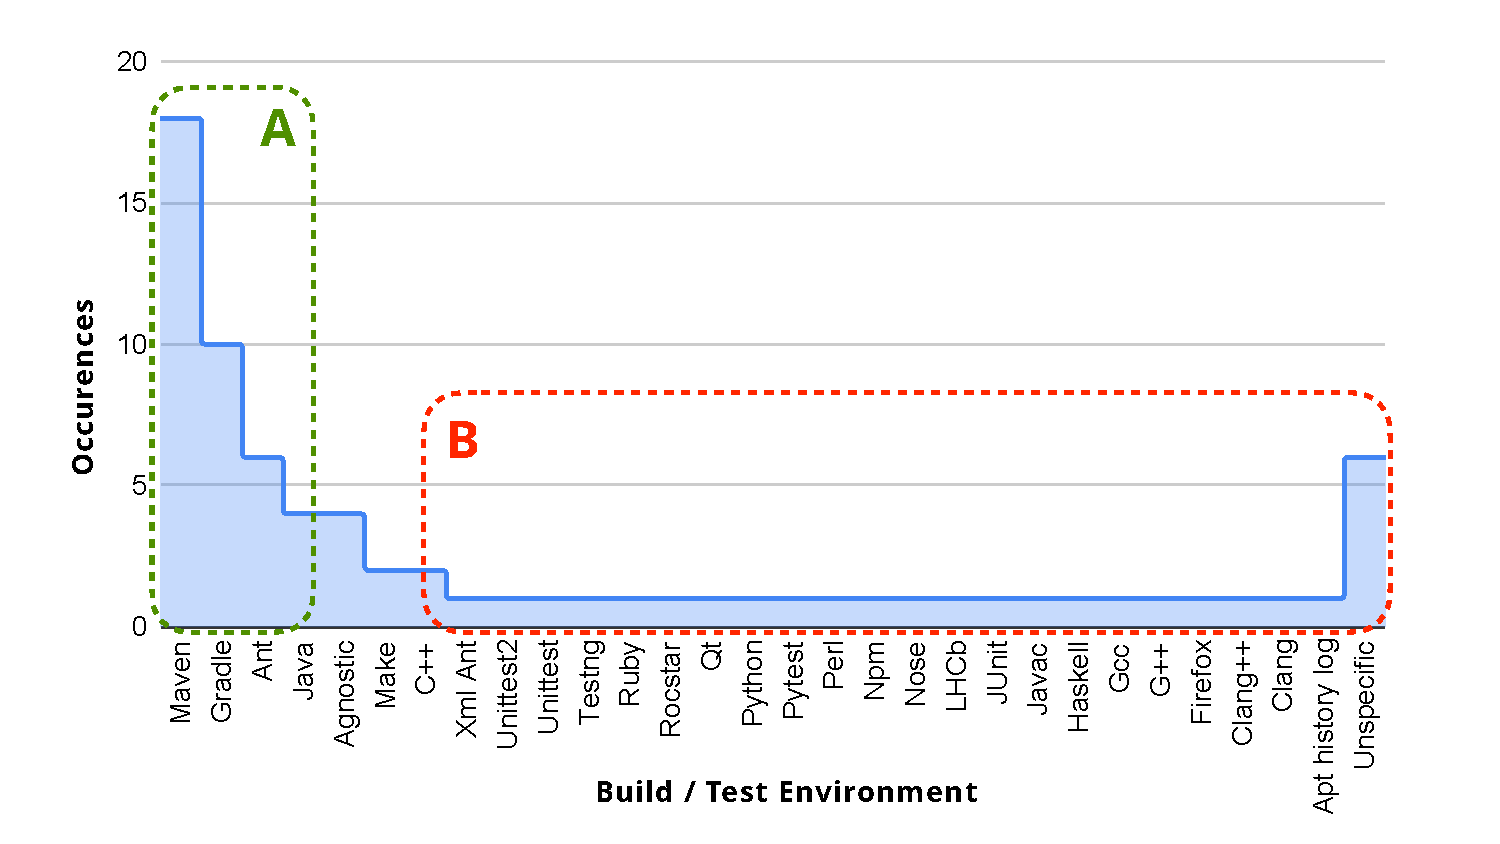
\includegraphics[width=\columnwidth, trim={1.5cm 0.4cm
		1.5cm 0.5cm},
		clip]{img/lit-sur/log_producer_annotated.pdf}
		\caption{Frequency of supported build tools.}
		\label{fig:litsur:log_producer}
\end{figure}

\subsection{Discussion}
\label{sec:lit-sur:discussion}
% tense: present

% ----- descriptive / general -----
Our literature survey shows that despite its relatively young age
(first mentioned in a paper in 2001, vast majority after
2016), \emph{build log analysis is already an established technique,}
with 61 works in different venues making use of it for a variety of
purposes.
We saw that various researchers analyze build logs, with the
logs often being the only available source for the
information they need for their studies~\cite{ren2018automated,
seo2014programmers,beller2017oops,zampetti2017open,rausch2017empirical}.

% ----- information RQ 1.1 -----
In regards to the information that is targeted, \emph{most build log
analysis approaches aim to retrieve the reason a build failed} by
targeting ``errors'' or ``failing tests.''
% which is what we also do in LogChunks
\emph{The majority of approaches retrieves specific chunks of
text from the logs.} Chunks are the overarching concept to
the almost equally much used categorization: one can deduce a
categorization from chunks, but not vice versa.

% ----- technique RQ 1.2 -----
\emph{Most log analysis is automated.} Automated approaches are
necessary because many studies target a large number of builds.
Works
that explicitly mention manual analysis of the logs, mostly
restrict themselves to few logs or take a ``representative sample to
make manual analysis feasible''~\cite{zolfagharinia2017not}.
We observed \emph{very little reuse of build log analysis tools},
even though works reported that
\emph{developing automated analysis tools requires a lot of effort}.
Urli et al.~\cite{urli2018design} strongly discouraged from parsing
build logs for information as it is ``too error prone,'' while other
works pointed to the effort of developing a custom tool.
We know from other research lines that regular expressions, the second
most popular way to analyze log files (\Cref{tab:litsur:techniques}),
are tedious to
maintain~\cite{michael2019regexes}.
In addition, we rarely saw works justifying why they use a certain
technique to analyze build logs as there is a general \emph{lack of
guidance on when to use which technique.}

% ----- kinds of build logs RQ1.3 -----
Several works noted the variety in log formats for different build
tools, which requires customizing build log techniques for
every supported build tool.
\Cref{fig:litsur:log_producer} shows that there are only a handful of
build tools whose build logs more than one study analyzed, mainly in
the Java ecosystem (area \circlenum{A}).
Many works target a unique build tool that did not appear in any other
study (area \circlenum{B}).
We follow that \emph{many seldomly-investigated
environments would benefit from the
existence of a more generic solution.}

The literature survey shows the need for
build log
analysis techniques that are \emph{automated},
\emph{build tool-agnostic}
and that a user can \emph{configure with little effort}.

% In most cases, \emph{researchers analyze build logs from open
% source projects}, obtained through Travis CI.
% In addition, we saw several works that targeted the logs of only
% one specific software project.

% ----- custom build tools -----

% What about the alternate solution, installing plugins to report
% precise data? Ie., maven plugins
% - Lots of effort
% - not a generic solution
% - how to analyze history where such plugins were not installed
% - unclear which information you want


% A downside of plugins, which are integrated into the CI flow similar to
% Deflaker by Bell et al.~\cite{bell2018deflaker}, is that they are unable
% to work on historic
% builds, i.e., before the moment they were being deployed and that if
% information has not been recorded from the beginning but turns out to
% be important, it is impossible to retrieve later.i

% \textbf{modifying the build output is not helpful}, as well as returning
% precise data through other documents than the log.
% This requires access to the build configuration, is also specific to
% the used build tool and prohibits the analysis of
% historical data.

% \textbf{ embed custom plugin discussion}
% %  very disconnected here
% From this, we follow: 1) there is a niche for custom parsers or even
% specialized plugins integrated into the build process to make
% post-factum
% parsing of logs redundant.
% Plugins  similar to, for example, the Maven plugin to report test
% executions Bell et al.
% % cite
% wrote, have the disadvantage of not being able to work on historic
% builds.
% 2) the large tail of seldomly-investigated environments would benefit
% from the existence of a more generic
% solution.

% We implement build tool agnostic build log analysis
% techniques, which are customized to a specific project by
% the training examples which the user provides.
% In addition, the \emph{LogChunks}~\cite{brandt2020logchunks}
% data set we chose for our evaluation covers a broad range of build
% environments.
% % Further, the training examples also specify the log chunk targeted
% by the
% % retrieval, which enable our chunk retrieval techniques to retrieve
% % a broad range of information from build logs.


% This task of retrieving specific chunks of text from the
% build logs can be solved by the chunk retrieval techniques we compare
% in this article.
% Our results can support researchers in choosing a
% suitable technique for their data set of build logs and the chunks
% they want to retrieve.
% By relieving them from building custom parsers
% we enable them to cover a much wider range of languages and build
% tools in their studies.

% Alt:
%\section{Analyzing Build Logs with Chunk Retrieval Techniques}
\section{Chunk Retrieval Techniques}
\label{sec:techniques}
% tense: past? except for general definitions / statements

In this section, we formally define the concept of chunk
retrievals from build logs.
Then, we motivate and present the choice of three such techniques that
we implemented and evaluated for this study.

% TOO Caro: Not sure what to do with this ...
%% In this section,
%% we propose three so-called \emph{chunk retrieval techniques},
%% which retrieve a specific substring (chunk)
%% from a build log
%% % TOO passive ....
%% The techniques we propose run automatically
%% and can be easily configured through examples.
%% % TOO this should go under characteristics and not be in an
% introduction
%% to the section ...
%% An example in this case consists of a build log together with the
%% chunk that should be retrieved.
%% A user---a developer or a researcher who wants to analyze
%% build logs---provides these examples, which are easy to
%% adapt whenever the analysis technique needs
%% to support new cases.


\subsection{Characteristics of Chunk Retrieval Techniques}
\label{sec:crt-characteristics}

With the term ``chunk retrieval technique,'' we refer to a way of
automatically extracting strings that appear literally in build
logs, i.e., techniques that do not aggregate, combine, or deduct
information.
We call such pieces of information in build logs
\emph{chunks}.

Generally, chunk retrieval techniques
can also be used to classify build logs, e.g.\, by checking
which substring was retrieved.
Therefore, they
cover the great majority of the types of log analysis we saw in
\Cref{sec:lit-sur:discussion}.

The techniques we investigate here do not require a formal lexer and
parser to analyze the entire structure of build logs, but focus on
ad hoc extracting just one specific piece of information per
configuration.

With the term \textit{configuration}, we abstract over the training
and parametrization that different techniques require in different
forms.
A configuration can be explicitly stated or implicitly derived
by learning through provided examples.
It is therefore a manual
specification of which information the chunk retrieval should target.
It also supplies the necessary information for the technique to
identify the targeted chunk in a build log.
Each chunk
retrieval technique has a specific \textit{granularity}, i.e.,\ the
smallest piece of text it can return (e.g., a line, or a word).
% The
% granularity might be adjustable by configuration.

\emph{Running a
chunk retrieval technique} means
% TODO what does it mean ``to apply?''
applying a fully configured
technique to a build log.
The technique then outputs a (possibly empty) list of substrings of the
build log text.

\subsection{Choice of Chunk Retrieval Techniques}

\begin{table*}[htb]
\centering
\caption{Chunk retrieval techniques.}
\begin{tabularx}{\textwidth}{@{}llXll@{}}
\toprule
Name & Acronym & Identification Technique & Granularity &
Configuration \\
\midrule
Program Synthesis by Example & PBE     & Regular expression program
& Character   & In/output examples	\\
Common Text Similarity	     & CTS     & TF-IDF \& cosine similarity,
expected number of lines & Line        & Output examples	   \\
Keyword Search		     & KWS     & Keywords, expected number of
lines			 & Line        & Keywords, context length  \\
Random Line Retrieval	     & RLR     & Random sample
& Line	      & Retrieval length	  \\
\bottomrule
\end{tabularx}
\label{tab:techniques}
\end{table*}


For this article, we designed and implemented three automated chunk
retrieval techniques.
Our findings of techniques in the literature
survey (~\Cref{sec:litsurresults} and \Cref{tab:litsur:techniques} in
particular) inspired the strategies that underlie them.
\Cref{tab:techniques} summarizes the techniques, which describe in detail
in the following.

Techniques based on custom parsers (\#1
in \Cref{tab:litsur:techniques}) are inadequate for our comparison,
since their creation is manual and one parser would never generalize
to the wide variety of build logs we are interested in.
The closest
we could come to the second most popular entry, regular expression, is
a technique to automatically derive them: in particular, we implement
a technique based on
\emph{Program Synthesis by Example (PBE)}.
It uses regular expressions internally, while simplifying their
development.

To work effectively with build logs, many humans anecdotally search
(``grep'') the logs for key phrases such as ``fail.'' Researchers often
resorted to such a strategy when doing manual analysis (\#2
in \Cref{tab:litsur:techniques}), describing it with the word ``scan''
or other paraphrases.
Imitating this ad hoc approach of searching for
specific strings, we automatize it as \emph{Keyword Search (KWS)}.

% TODO Caro, can you check this? Also I did not find any literature
% references to CTS.
It does not seem to be a common technique?
% Where does the name come from then?
Finally, from the fields of information retrieval (IR) and natural
language
processing (NLP), we leverage a
\emph{Common Text Similarity (CTS)} approach.
The inspiration behind it---apart from literature indicating the use
of IR and NLP (\Cref{tab:litsur:techniques})--- is that the relevant,
failing parts of build logs often looks similar to each other, even if
the exact failure reason might differ.

\subsection{Program Synthesis by Example (PBE)}
The idea behind \emph{Programming by Example} is to automatically
generate a program, by capturing the
intent of the user through examples that the user provides.
Leveraging this approach, we designed a chunk retrieval technique
for build logs.
The \emph{PROSE library}~\cite{prose2019webpage} forms the basis for
our implementation.
This library builds on the generic program synthesis framework
\emph{FlashMeta}~\cite{polozov2015flashmeta:} and the specialized
text extraction DSL \emph{FlashExtract}~\cite{le2014flashextract:}.
% Both enable \emph{PROSE} to synthesize regular expression programs
% consistent~\cite{mitchell1982generalization} with a set of in-
% and output examples.
% The usage of example enables the user to configure a chunk
% retrieval without understanding the whole structure of
% the build log.

\subsubsection{Configuration}
In- and output example pairs are the main driver of PBE;
The \emph{input} is the full text of the build log file.
The \emph{output} is
a substring of the log file text, representing the
substring that the synthesized program should retrieve when
given the corresponding input file.
One or multiple examples, the
training set, \emph{configure} a specific chunk retrieval with PBE:
they define the chunk of a build log that should be retrieved.
The PROSE program synthesis then tries to construct a program
consistent with all training
examples~\cite{mitchell1982generalization}.
If PROSE cannot synthesize a program, e.g.,\
because the required regular expression
is too complicated to be synthesized, PBE returns the
error message ``no program found.''

\subsubsection{Application}
A run of PBE takes a build log file as input and applies the
synthesized regular expression program.
It then returns the substring
of the build log matched by the program.
If the program finds no match because the analyzed build log
does not contain the structure that the training examples define,
PBE returns the error message ``no match found.''

\subsection{Common Text Similarity (CTS)}
Text Similarity approaches are widely used to filter unstructured
textual software artifacts~\cite{runeson2007detection,
marcus2005recovery,antoniol2002recovering,mccarey2006recommending}.
These approaches fall into the broader area of information retrieval
techniques, which several of the works from our literature survey
used to analyze build logs.
Similar to these approaches, we designed a chunk retrieval
technique that
retrieves those lines from a build log which are most
similar to the specified examples.

\subsubsection{Configuration}
To configure CTS we chose to use the same concept of examples as for
PBE: lines of the targeted chunks from the training examples define
the search query.
Using a Vector Space
Model~\cite{schutze2008introduction} (VSM), an algebraic model for
representing textual documents, we encode each line as a separate term
vector.
The terms that make up the dictionary are simply all words
that appear in the example logs, where we separate words by spaces.
% TODO Caro: complete above sentence if we separate by anything else
The vectors comprise points counting
how many times a word out of the dictionary appears in the specific
line at hand.

The idea behind a representation in the VSM is that text lines as more
similar if they contain the same words in similar frequencies,
making their term vectors point in a similar direction in vector
space.
We use \emph{cosine similarity}~\cite{korenius2007principal}
to calculate the angle between two term vectors.
The smaller the
angle between term vectors is, the more similar are the corresponding
lines.

To improve the similarity calculation, we prune very often or
very rarely appearing words.
Finally, the
algorithm weighs the vectors using \emph{term frequency-inverse
document frequency (TF-IDF)}, a best practice for natural
language queries~\cite{lee1997document}.

\subsubsection{Application}
To retrieve the desired information from a build log, we encode every
line of the input build log in VSM.
The algorithm calculates the cosine
similarity to compare each line of the
build log with each line of the search query.
After summing up the
similarities of each build log line to all search query lines, we sort
the build log lines in decreasing similarity.
The average number of
lines in the chunks of the training examples determines how many of
the most similar lines our approach returns as the output of the retrieval
run.

\subsection{Keyword Search (KWS)}
When developers scavenge for a specific piece of information within a
large amount of unstructured information, a first ad hoc approach they
use is to search for related keywords.
%% TODO Caro: I took this out as it interrupts reading flow.
Do you
%% agree?
%% Indeed, this was one of the
%% most common approaches we took when searching for the reason a build
%% failed while creating the \emph{LogChunks} data
%% set~\cite{brandt2020logchunks}.
To investigate the performance of this approach, we designed a chunk
retrieval technique mimcing this human behavior based on keyword
search.

\subsubsection{Configuration}
A set of keywords configures the chunk retrieval with KWS\@.
To better
compare KWS with PBE and CTS, we also configure it through examples.
% TODO (resolved) associate is very abstract and tells us
% less about what is going on than the new version
From each example, we extract a list of keywords that we hope should
also appear in, or close to, the targeted chunk of new input.
Finally, we merge the lists from all examples to build one unified
list of the most commonly occurring keywords for the search with KWS.

\subsubsection{Application}
For a retrieval run, we take an entire build log file as input and
search for all exact occurrences of the search keywords.
As keywords are
often not directly describing the desired information, but rather
appear close to it, KWS also retrieves a context of lines
around the found keyword.
The number of surrounding lines retrieved is
the average number of lines in the chunks of the training examples.

\subsection{Random Line Retrieval (RLR)}
\label{sec:expl-rlr}
To fully comprehend how difficult the task of build log analysis really
is without any a priori knowledge, we include a comparison with a
baseline of
picking lines at random from the build log.
RLR mimics the
situation of guessing blindly which lines are interesting.
The only configuration option for RLR is the number of lines it should
retrieve.
For a comparison to the other techniques (whose number of
% TODO Caro: but wait, this is not really true for KWS, right?
returned lines is dynamic), we configure RLR to return the average
number of lines in the chunks of the training examples.

\subsection{Concrete Example}
\label{sec:crt-example}

\lstset{escapeinside=//}
\begin{figure}[tbp]
  \centering
\begin{subfigure}[tbp]{\columnwidth}
  \begin{lstlisting}[breaklines=true,frame=tlr]
FAILURE: Build failed with an exception.

* What went wrong:
  \end{lstlisting}
  \vspace{-\baselineskip}
  \begin{lstlisting}[backgroundcolor=\color{Cerulean!60},breaklines=true,frame=rl]
Could not determine the dependencies of task ':app:jacocoTestDebugReport'.
> Task with path 'testDebug' not found in project ':app'.
  \end{lstlisting}
  \vspace{-\baselineskip}
  \begin{lstlisting}[breaklines=true,frame=blr]

* Try:
  \end{lstlisting}
\end{subfigure}\hspace{\fill}
\begin{subfigure}[tbp]{\columnwidth}
  \centering
  \begin{lstlisting}[breaklines=true,frame=tlr]
FAILURE: Build failed with an exception.

* What went wrong:
  \end{lstlisting}
  \vspace{-\baselineskip}
  \lstinputlisting[backgroundcolor=\color{Cerulean!60},breaklines=true,frame=rl]{listings/chunk1.txt}
  \vspace{-\baselineskip}
  \begin{lstlisting}[breaklines=true,frame=blr]

* Try:
  \end{lstlisting}
    \caption{Two examples of log chunks explaining why an Android
  build failed.}
  \label{lst:chunk-example}
\end{subfigure}

\begin{subfigure}[tbp]{\columnwidth}
  \begin{lstlisting}[breaklines=true,frame=tlr]
=== RUN   TestSeparator
  \end{lstlisting}
  \vspace{-\baselineskip}
  \lstinputlisting[backgroundcolor=\color{Cerulean!60},breaklines=true,frame=rl]{listings/chunk2.txt}
  \vspace{-\baselineskip}
  \begin{lstlisting}[breaklines=true,frame=blr]
=== RUN   TestGenerateHTML
  \end{lstlisting}
  \caption{Example of a log chunk showing a linter error.}
  \label{lst:chunk-example-3}
\end{subfigure}

\caption{Exemplary log excerpts.}
\label{lst:logexamples}
\end{figure}

\lstset{language=caml, morekeywords={StartExtraction, RegexPosition,
RegexPair,
  EndExtraction}, keywordstyle=\bfseries\color{black}}
\begin{figure}[tbp]
  \centering
  \lstinputlisting[breaklines=true]{listings/prose.txt}
  \caption{Simplified regular expression produced by PBE when trained
  with examples from \Cref{lst:chunk-example}.}
  \label{lst:prose-program-simplified}
\end{figure}


In this section, we illustrate how the different chunk retrieval
techniques work practically on the example of the build logs
in \Cref{lst:logexamples}.
Marked in blue in \Cref{lst:logexamples}
are the chunks we target.
They contain the information on why the
corresponding build failed.
\Cref{lst:chunk-example} shows two excerpts
from Android build logs.
The chunk to be retrieved starts after a
colon and a line separator and before a capital letter.
It ends
before two line separators.
All these characteristics are consistent
with the two example chunks
from \Cref{lst:chunk-example}.
\Cref{lst:chunk-example-3} is very
different.
For example, it does not have the two extraneous newlines
after the chunk.

% TODO Caro: I like this explanation of structural categories and
% would leave it here (slightly adapted), but I think
% struct.
categ.
should be mentioned earlier -- not sure if you know a
% better place, but how about sec.
3.1? i don't think people should
% have to read an example section -- which they might skip -- to
% get to know of this important concept!

When we train PBE with the two examples from \Cref{lst:chunk-example},
it produces a regular expression program similar to the one presented
in
\Cref{lst:prose-program-simplified}.
This shows that the characters structuring the text around the chunk are
crucial for regular expressions to identify a log chunk.
In fact, if we add the third example from
to the training set (which has a
different structural representation),
PBE is not able to synthesize a program anymore and returns
``\texttt{no program found}.''
We later express this difference in structural representation through
separating log chunks into \emph{structural categories}.
The chunks from \Cref{lst:chunk-example}
are in the \emph{same structural category}, while the chunk from
\Cref{lst:chunk-example-3} is in a
\emph{different structural category}.

CTS will rank the lines from an analyzed build log which are most
similar to the chunks in the training examples
from \Cref{lst:chunk-example}.
It will then return the two lines ranked highest, as the chunks in
the training examples have on average 2.0 lines.
% TODO Caro: How well does it deal with the third example?

Keywords that appear in or close to the chunk within
the build log configure the technique KWS\@.
For the examples from \Cref{lst:chunk-example} these could be
``FAILURE,'' ``wrong,'' or ``failed.''
The example from \Cref{lst:chunk-example-3} could be found
by searching for ``FAIL.''
If we train KWS with all three examples and the aforementioned
associated keywords, it would search for the three keywords from
\Cref{lst:chunk-example}, as they appear twice---most often within
the training set of three examples.

\subsection{Tool Implementation}
For the comparison study, we implemented the three chunk retrieval
techniques described in this section and a unifying interface.
We implemented PBE in C\# based on the Microsoft PROSE
library~\cite{prose2019webpage} and CTS, KWS, and RLR using
R and the {\tt text2vec} library~\cite{text2vec2019webpage}.

\section{Empirical Comparison Study}
\label{sec:study}

% TODO: decide if keep or redo
% if keep, Caro do noted improvements
\begin{figure*}[tb]
	\centering
	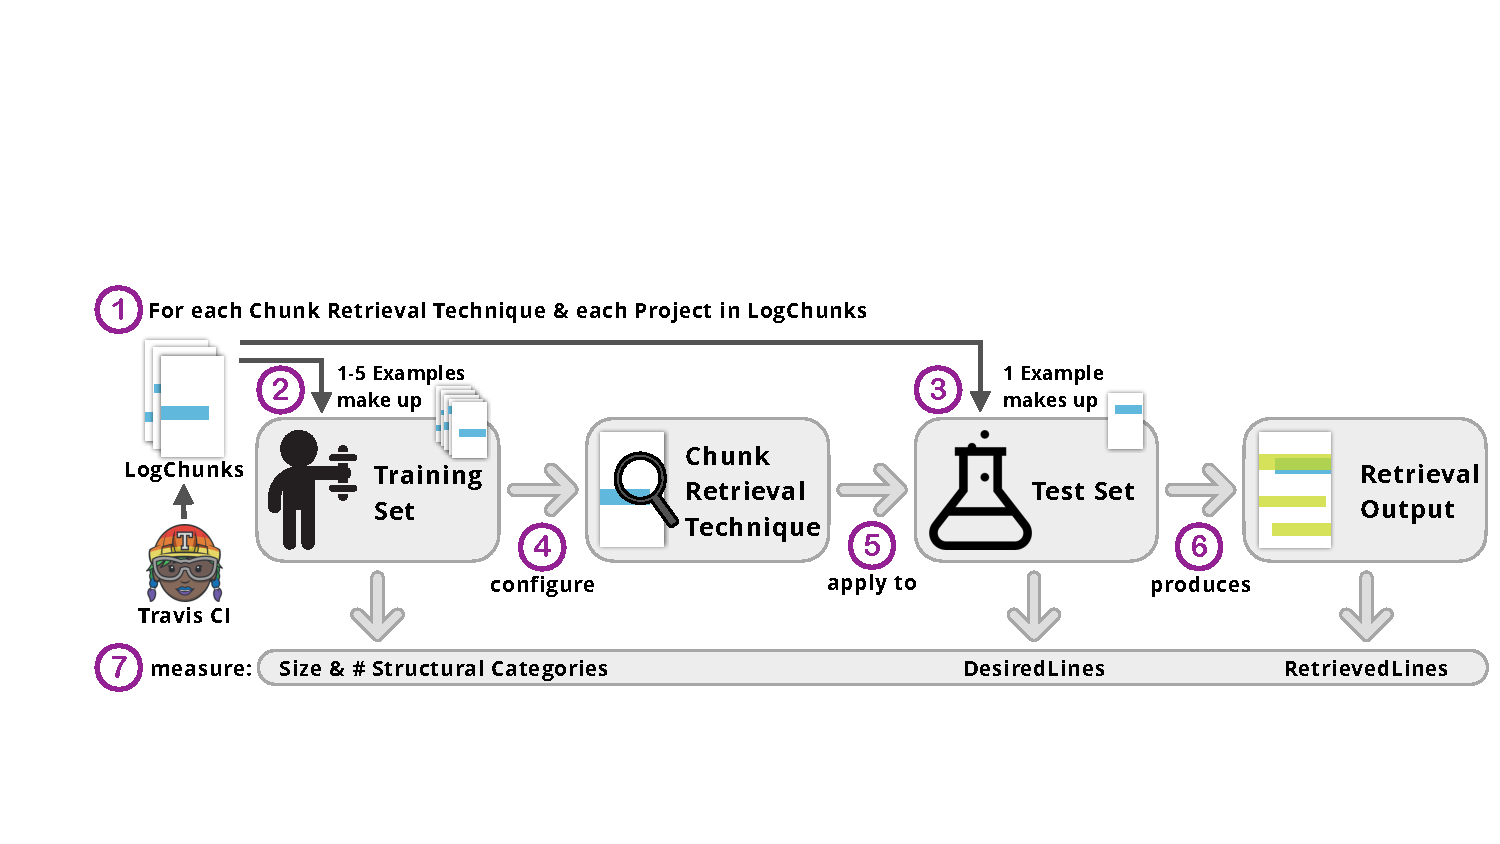
\includegraphics[width=\textwidth, trim={1.6cm 2.5cm 0.2cm 4.8cm},
  clip]{img/study.pdf}
	\caption{Study design of the technique comparison study.}
	\label{fig:study}
\end{figure*}

In the literature survey, we noted that previous work seemed to choose
a log analysis technique arbitrarly and that is a lack of guidance on
when to use which technique.
% add (see \Cref{sec:lit-sur:discussion}) ?
To address this, in this section, we conduct an empirical study
comparing the three novel chunk retrieval techniques we presented in
\Cref{sec:techniques}.

In particular, we are interested in how many examples a technique
should be trained with (\textbf{RQ2.1}),
how similar the structural representation of the targeted log chunks
has to be (\textbf{RQ2.2}), and how reliable the quality of the
produced retrievals is (\textbf{RQ2.3}).
This leads us to the following research questions:

\begin{simplebox}[minipage boxed title*=-1.5cm,
attach boxed title to top center={yshift=-6mm}]
{\textbf{RQ2:} How do build log analysis techniques compare?}
\begin{itemize}[leftmargin=1.2cm]
  \item[\textbf{RQ2.1:}] How many examples does a technique need to
  perform best?
  \item[\textbf{RQ2.2:}] How structurally similar do the examples
  need for a technique to be applicable?
  \item[\textbf{RQ2.3:}] How accurate are the retrievals of a technique?
\end{itemize}
\end{simplebox}

In the following, we first introduce the data set we created for this
study, and then describe the study design and its
results.

\subsection{LogChunks Data Set}
\label{sec:logchunks}
To conduct the study in this paper, we created the
\emph{LogChunks} data set~\cite{brandt2020logchunks}.
We collected 797 build logs that
from 80 GitHub projects and 29
programming languages on Travis CI, the most-used source of build logs
according to our literature survey.
This wide variety of projects and the large number of different build
tools they employ enables us to measure the generic
applicability of chunk retrieval techniques.

For each build log in \emph{LogChunks}, we manually marked
the chunk that describes why the build
failed---the information targeted by most of the works in our
literature survey (see \Cref{sec:lit-sur:discussion}).
To be able to configure the keyword search technique,
% TODO (resolved) the data set cannot associate anything
we associated each chunk in the data set with keywords that we
would use to search for the selected chunk within the log.
In
addition, we categorized the log chunks according to their format
within the log.
% TODO Are surrounding markings really the only structural
% category element? I doubt that
If the chunks were, for example, surrounded by the same markings
within the log, we assigned them the \emph{same structural category},
as described in \Cref{sec:crt-example}.

% TODO what does this refer to here? Make it clearer.
%It would refer to the strcutrual categories but
% that is already in the list?

% TODO couldn't it also be chunks? why corresponding?
As explained in \Cref{sec:crt-characteristics}, examples are the basic
unit by which we configure each technique.
The full build log text,
chunk(s), search keywords, and the assigned structural categories make
up one \emph{example} in \emph{LogChunks}.


\subsection{Study Design}

In the following, we explain the individual steps of our study design
and introduce the metrics that
we measure to answer RQ2.

% TODO Didn't we above define ``run'' instead of apply?
% Shouldn't we then also use it here?
% TODO wow, this starts already super confusing
We run each of the three chunk retrieval techniques
on all of the 80 projects in
\emph{LogChunks} \circlenum{1}.
For each project, we select training sets of size 1, 2, \dots 5
\circlenum{2}.
We vary the training set size to measure how many examples we need to
confidently configure a technique.
The training set is so small because the examples have to be
manually created by a user.
A larger training set would oppose our goal of providing techniques
that can be configured with little effort
(see \Cref{sec:lit-sur:discussion}).

The test set consists of an example based on the build log produced
chronologically after the build logs in the training set \circlenum{3}.
This way, we train on examples from past build logs and test on
more recent logs.
% We chose a test set size of 1, as users of the techniques
% should receive reliable results on every build log they analyze.
% M: and why is this important? Doesn't everyone want such stability
%of results?
% C: motivation why only one test example.
% we can also leave that out
% and answer if we are asked about it

In the next step, we configure a chunk retrieval technique with
the examples from the training set \circlenum{4} and apply the technique
to the
training set \circlenum{5}, which produces the retrieval output
\circlenum{6}.

Based on this, we collect retrieval performance measurements \circlenum{7}
for
the size of the training set (\textbf{RQ2.1}),
the number of structural categories in the training
set (\textbf{RQ2.2}),
the lines of the retrieval output ($\mathit{RetrievedLines}$),
and the oracle: the output defined in the test example
($\mathit{DesiredLines}$).
From these we calculate accuracy metrics (\textbf{RQ2.3}):

\vspace{0.2cm}
\begin{itemize}[leftmargin=0.4cm] \itemsep1em
	\item $|\mbox{True\ Positives}| = \mathit{DesiredLines} \cap
	\mathit{RetrievedLines}$ \vspace{0.2cm}\\
	True positives are lines that appear both in the output of a
	technique as well as the chunk defined in the
  test example.

	% What about when a line is replicated twice?
	% I.e., Are line numbers part of this? => no.
	% not checked, but if lines are identical they also contain
	% the same information so if someone asks we can defend I think

	\item $\mbox{Precision} = \dfrac{|\mathit{True\
	Positives}|}{|\mathit{RetrievedLines}|}$ \vspace{0.21cm} \\
	Precision of a chunk retrieval describes which proportion of
	the retrieved lines were actually desired.

	\item $\mbox{Recall} =
	\dfrac{|\mathit{True\ Positives}|}{|\mathit{DesiredLines}|}$
	\vspace{0.2cm} \\
	Recall of a chunk retrieval describes which proportion of the
	desired lines were retrieved.

	\item $\mbox{F$_{1}$-score} = 2 \cdot \dfrac{\mathit{Precision}
	\cdot \mathit{Recall}}{\mathit{Precision} + \mathit{Recall}}$
	\vspace{0.2cm}\\
	In addition, we calculate the F$_{1}$-score, the harmonic mean
	of precision and recall.
  We prefer F$_{1}$ to other aggregate
	measures such as accuracy because of the
	``needle-in-the-haystack'' scenario, we want to avoid bloating
	our results by correctly not finding lots of irrelevant log
	lines.

	% actually that is now giving recall another (nicer) name
	% improved if we just talk about recall later?
	\item Successful retrieval = $\mathit{true}\ \mathit{iff}\
	\mathit{Recall} = 1, \vspace{0.1cm}\\$
	Partially successful retrieval = $\mathit{true}\ \mathit{iff}\
	0<\mathit{Recall}<1, \vspace{0.1cm}\\$
	Unsuccessful retrieval = $\mathit{true}\ \mathit{iff}\
	\mathit{Recall} = 0, \vspace{0.1cm}$

	We define a successful retrieval as one where all desired
	lines were extracted, therefore when recall is one.
	A retrieval is partially successful if at least some of the
	desired lines were extracted,
	and if the retrieved lines contain none of the desired lines
	a retrieval was unsuccessful.
\end{itemize}

\subsection{Results}
The empirical comparison study yielded diverse results for the
different chunk retrieval techniques
In this section, we first present the results for each chunk retrieval
technique separately.
Afterwards, we compare the three techniques with each other and with a
random baseline.

\subsubsection{Program Synthesis by Example (PBE)}
\label{sec:r:pbe}

\begin{figure}[tbp]
		\centering
		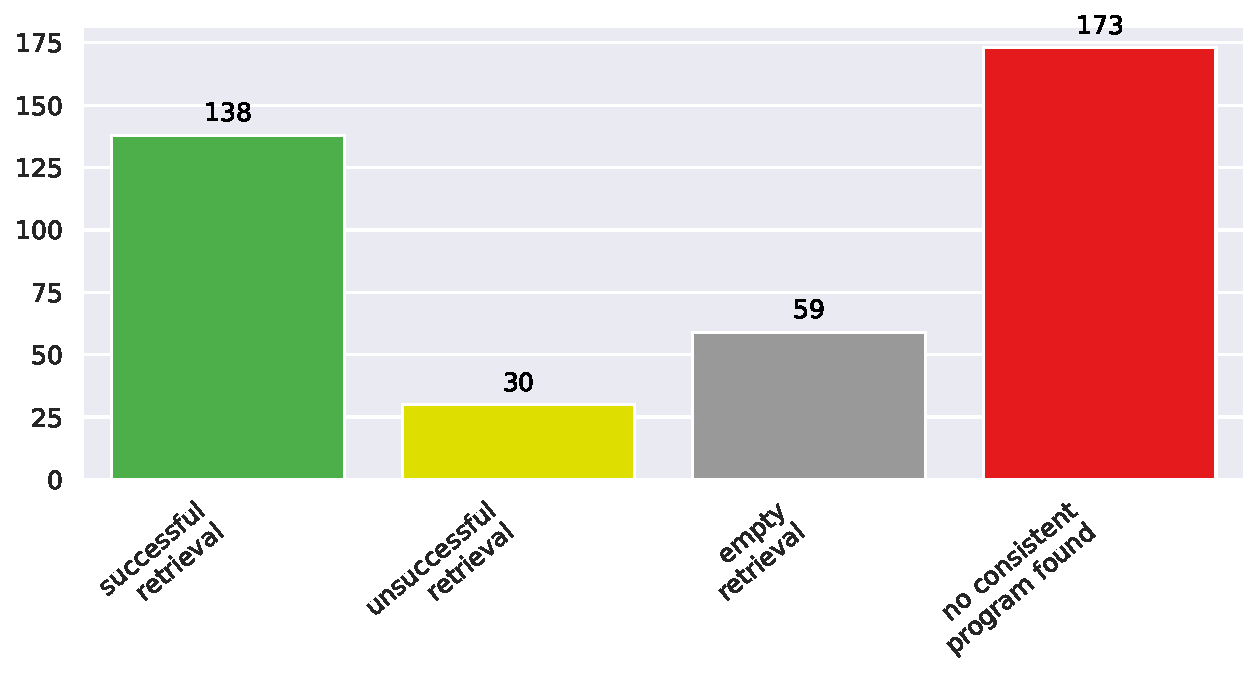
\includegraphics[width=\columnwidth,
		clip]{img/big-study/failure-reason-pbe.pdf}
		\caption{High-level results of chunk retrieval with
		Program Synthesis by Example (PBE).}
		\label{fig:failure-reason-PBE}
\end{figure}

\lstset{
  language=,
  morekeywords={Test, Output, Desired},
  keywordstyle=\textbf,
	frame=single
}
\begin{figure}[tbp]
  \centering
\begin{subfigure}[b]{\columnwidth}
  \begin{lstlisting}[breaklines=true,frame=tlr]
[0K$ test/sass-compile-tester.sh
  \end{lstlisting}
  \vspace{-\baselineskip}
  \lstinputlisting[backgroundcolor=\color{Yellow!60},breaklines=true,frame=rl]
	{listings/chunk3.txt}
  \vspace{-\baselineskip}
  \begin{lstlisting}[breaklines=true,frame=blr]
	from line 5 of sass/components/_all.sass
  \end{lstlisting}
	\caption{Actual chunk retrieval output ($RetrievedLines$
	in yellow).}
	\label{lst:pbe-part-success-output}
\end{subfigure}

\begin{subfigure}[b]{\columnwidth}
  \begin{lstlisting}[breaklines=true,frame=tlr]
[0K$ test/sass-compile-tester.sh
  \end{lstlisting}
  \vspace{-\baselineskip}
  \lstinputlisting[backgroundcolor=\color{Cerulean!60},breaklines=true,frame=rl]
	{listings/chunk3.txt}
  \vspace{-\baselineskip}
  \begin{lstlisting}[backgroundcolor=\color{Cerulean!60},breaklines=true,frame=rl]
	from line 5 of sass/components/_all.sass
	from line 6 of bulma.sass
  \end{lstlisting}
  \vspace{-\baselineskip}
  \begin{lstlisting}[breaklines=true,frame=blr]
  Use --trace for backtrace.
  \end{lstlisting}
	\caption{Targeted chunk ($DesiredLines$ in blue).}
	\label{lst:pbe-part-success-desired}
\end{subfigure}
  \caption{Example of a partially successful retrieval
  (PBE retrieved only
  two of the four targeted lines).}
  \label{lst:pbe-partially-successful}
\end{figure}

\begin{figure*}
\centering
    \textbf{Program Synthesis by Example (PBE)}\par\medskip
\begin{subfigure}[b]{\columnwidth}
		\centering
		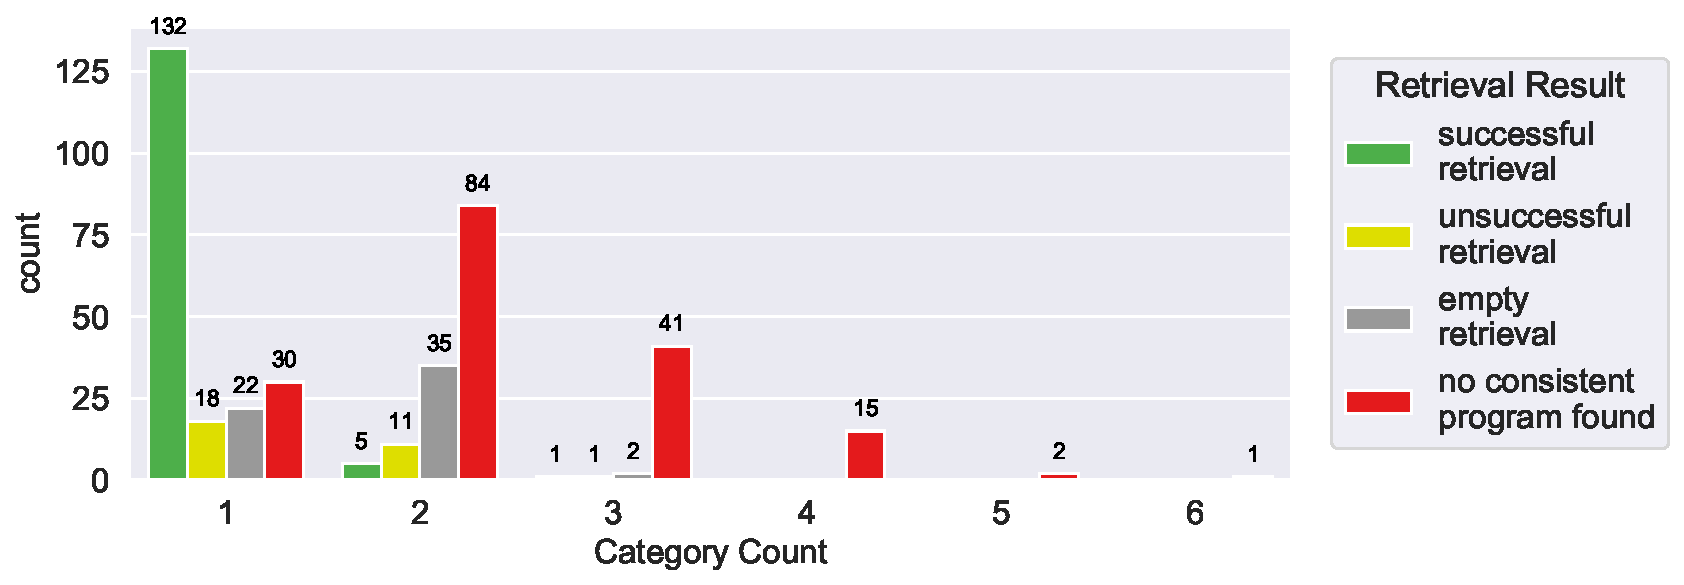
\includegraphics[width=\columnwidth,
		clip]{img/big-study/failure-reason-categorycount-PBE.pdf}
				\caption{Successfulness of retrieval
				compared by structural category count
				in training and test sets.}
		\label{fig:failure-reason-categorycount-PBE}
\end{subfigure}\hspace{\fill}
\begin{subfigure}[b]{\columnwidth}
		\centering
		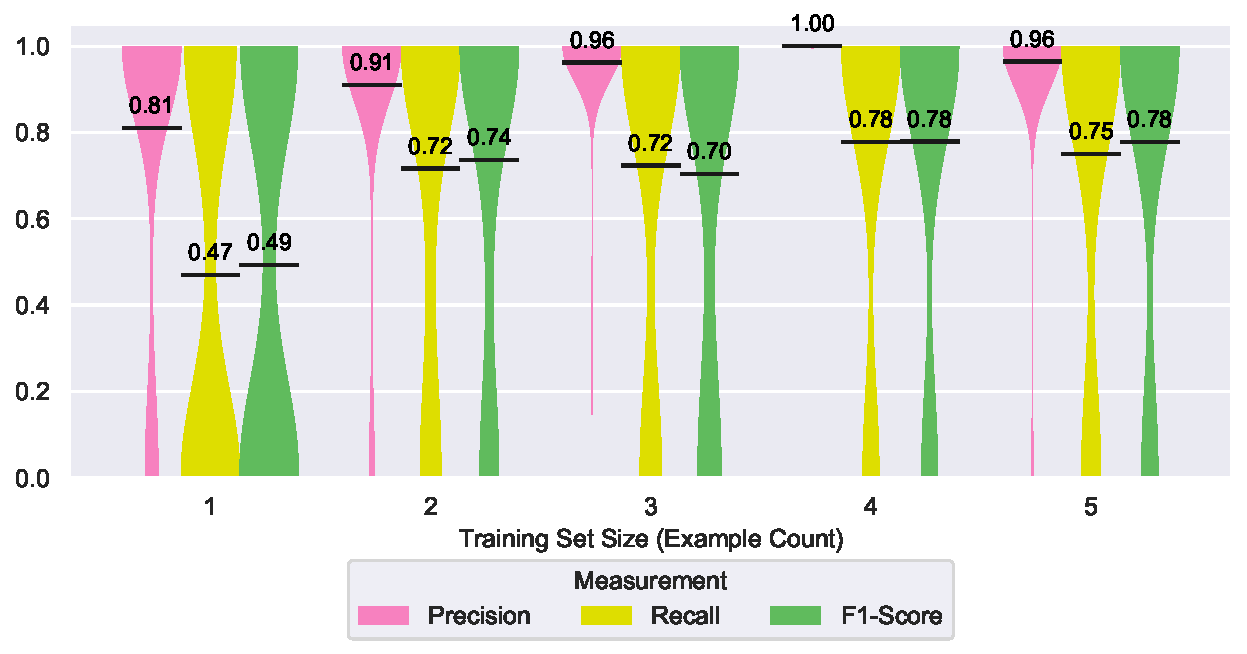
\includegraphics[width=\columnwidth,
		clip]{img/big-study/recall-precision-examplecount-sythesisworked-PBE.pdf}
				\caption{Precision, recall, and
				F$_{1}$-score when PBE could synthesize
				a consistent program compared with the
				size of the training set.}
		\label{fig:recall-precision-examplecount-sythesisworked-PBE}
\end{subfigure}
\caption{Results of chunk retrieval with Program Synthesis by Example
(PBE).}
\end{figure*}

% actually, we could cut this figure and move it's explanation
% to the next one (this is an aggregation of the next one)
% however, having them separate eases the entry into the results a bit
% and we have explanation of the categories before the more complicated
% aspect of the change with more structural categories
\Cref{fig:failure-reason-PBE} shows the results of chunk
retrieval with PBE.
It shows how many of the retrieval runs were successful,
partially successful, or unsuccessful,
as well as the number of runs where the
synthesized program did not match on the analyzed build log or where
no program could be synthesized.
% The last two results stem from the regular expressions and their
% synthesis, therefore only apply to PBE.
Out of the 400 runs, 5 per each one of the 80 projects,
PBE extracted all desired lines successfully in 138 cases.
In 18 cases, the synthesized program only extracted a
subset of the desired lines, while in 12 cases it extracted none of
the desired lines.
For the 18 partially successful runs, the average recall
was 47\%.
\Cref{lst:pbe-partially-successful} shows an example of such
a partially successful retrieval.
In it, the synthesized program only
retrieved two (\Cref{lst:pbe-part-success-output})
of the four (\Cref{lst:pbe-part-success-desired}) targeted lines.
In 59 cases, PBE could synthesize a regular expression program, though
the program did not match on the test build log.
In 173 of the 400 cases
could PROSE not synthesize a program consistent with all of the training
examples.

\Cref{fig:failure-reason-categorycount-PBE} shows how
the results of PBE
runs depend on the number of structural categories in the training and
test examples.
% It shows the categories from above change depending on how many
% structural categories are present.
The figure demonstrates that program synthesis mostly
returns exactly the desired output when there is only one
structural category present in the training and test examples.
However, when
two or more structural categories are simultaneously present,
PROSE could in most cases not synthesize a program.
For four or more present
categories PROSE could never synthesize a consistent program.

Zooming in on only the 227 runs where PBE could synthesize a program,
\Cref{fig:recall-precision-examplecount-sythesisworked-PBE}
presents violin plots and averages of the precision, the recall
and the F$_{1}$-score
of these runs compared with the number of examples in the training set.
When the training set
size increases from one to two, recall, and F$_{1}$-score increase by
about 25\%, precision increases by about 10\%.
For two or more
training examples, recall, and F$_{1}$-score stay around 75\% and
precision around 96\%.

\subsubsection{Common Text Similarity (CTS)}
\label{sec:r:cts}

\begin{figure*}
\centering
    \textbf{Common Text Similarity (CTS)}\par\medskip
\begin{subfigure}[tb]{\columnwidth}
		\centering
		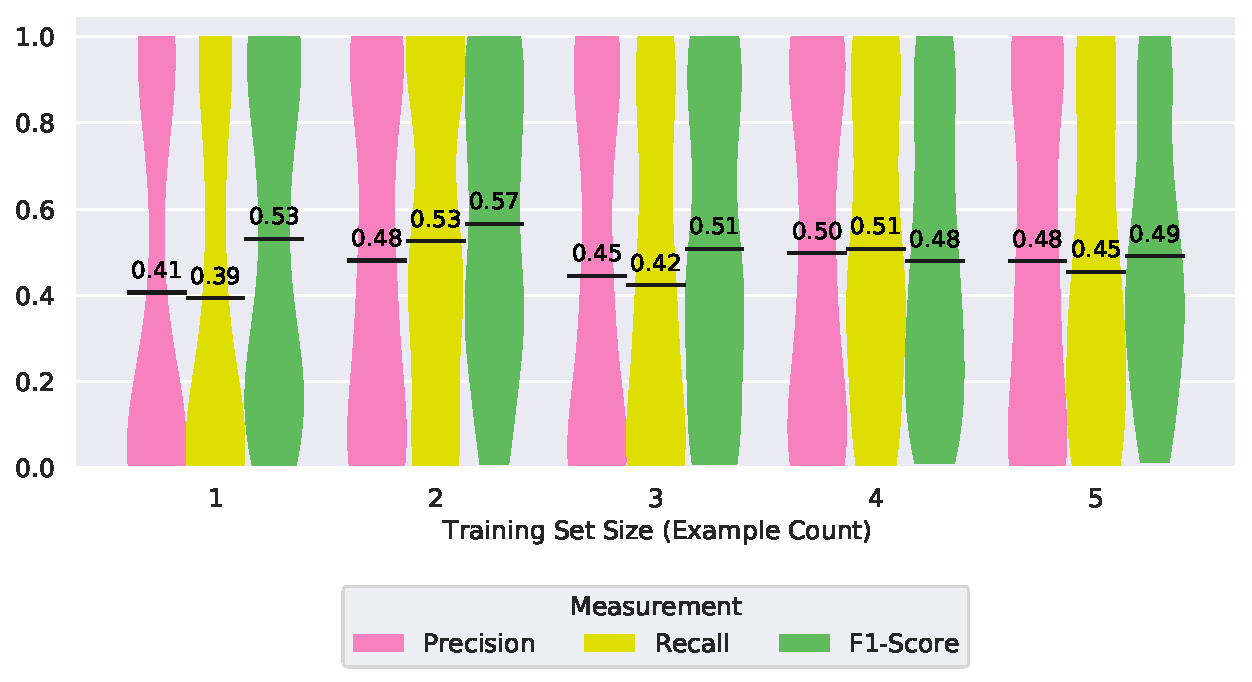
\includegraphics[width=\columnwidth,
		clip]{img/big-study/recall-precision-examplecount-CTS.pdf}
		\caption{training set size.}
		\label{fig:recall-precision-examplecount-CTS}

\end{subfigure}\hspace{\fill}
\begin{subfigure}[tb]{\columnwidth}
		\centering
				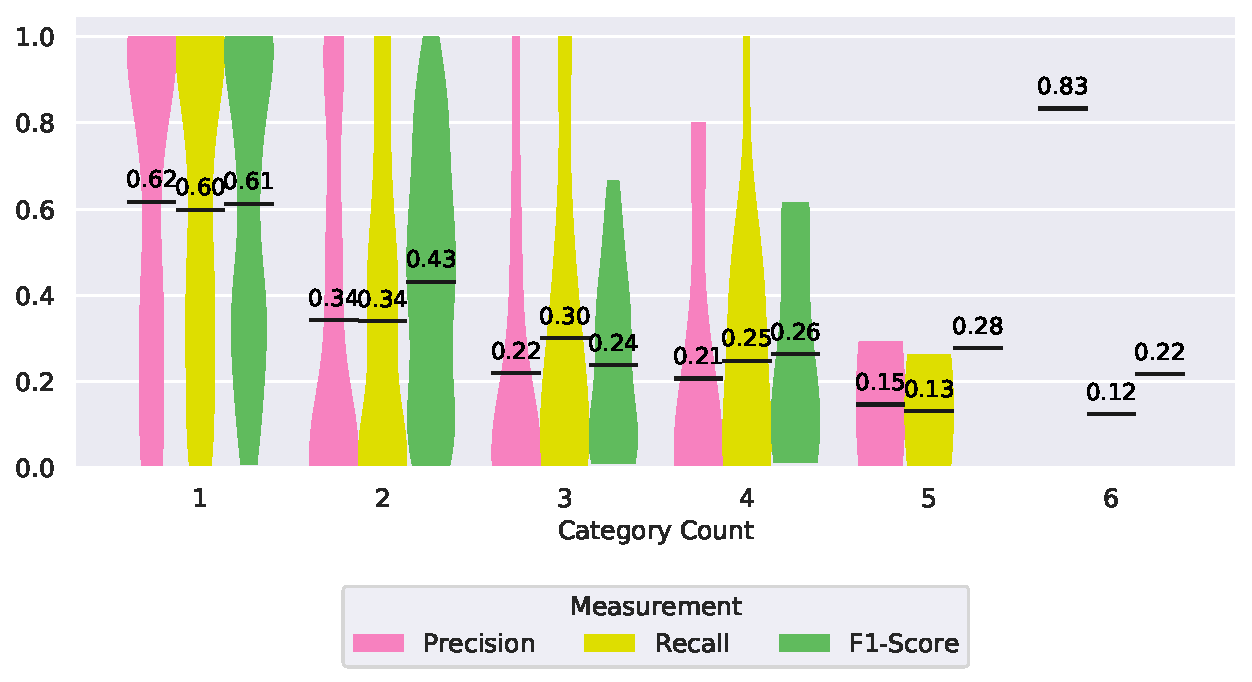
\includegraphics[width=\columnwidth,
				clip]{img/big-study/recall-precision-categorycount-CTS.pdf}
		\caption{structural category count
		in training and test set.}
		\label{fig:recall-precision-categorycount-CTS}
\end{subfigure}
\caption{Precision, recall, and F$_{1}$-score of chunk
retrieval with Common Text Similarity (CTS) compared by \ldots}
\label{fig:results-CTS}
\end{figure*}

% The following sections are each quite short...
% we could merge them, but then it loses consistency with the other
% result subsections where each plot gets an own paragraph
\Cref{fig:results-CTS} shows violin plots
of the precision,
recall, and F$_{1}$-score of the chunk retrieval runs with CTS.
The black horizontal lines show the average of these measurements.
For some measurements, the violin plot is not visible because there is
only one available data point or all data points have the same value.

\Cref{fig:recall-precision-examplecount-CTS} presents the
measurements for an
increasing number of training examples.
When using one to five
training examples, the size of the training set has no noticeable
influence on precision, recall or F$_{1}$-score of the chunk retrieval
with CTS.

\Cref{fig:recall-precision-categorycount-CTS} shows the
measurements for an increasing number of structural categories in the
training and test examples.
With increasing category count, precision,
recall, and F$_{1}$-score decrease.
% Especially for more than four
% categories present we have no chunk retrieval runs where all desired
% lines were extracted.

\subsubsection{Keyword Search (KWS)}
\label{sec:r:kws}
\begin{figure*}
\centering
    \textbf{Keyword Search (KWS)}\par\medskip
\begin{subfigure}[b]{\columnwidth}
		\centering
		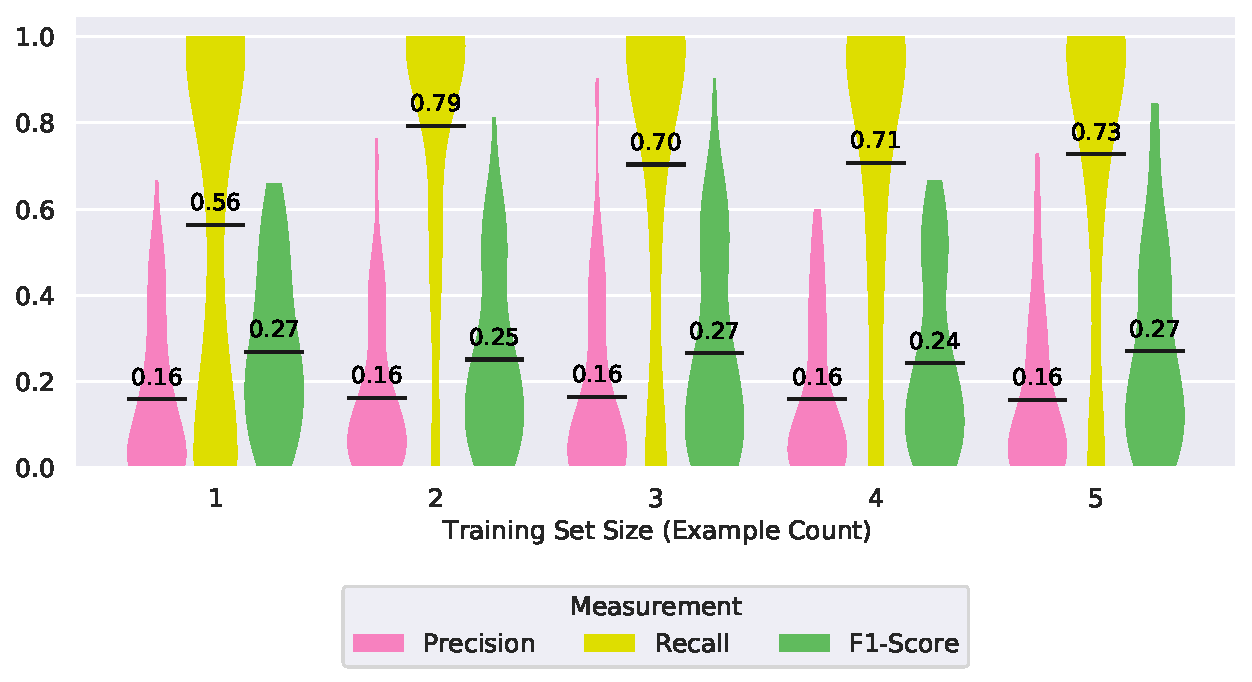
\includegraphics[width=\columnwidth,
		clip]{img/big-study/recall-precision-examplecount-KWS.pdf}
		\caption{training set size.}
		\label{fig:recall-precision-examplecount-KWS}
\end{subfigure}\hspace{\fill}
\begin{subfigure}[b]{\columnwidth}
		\centering
		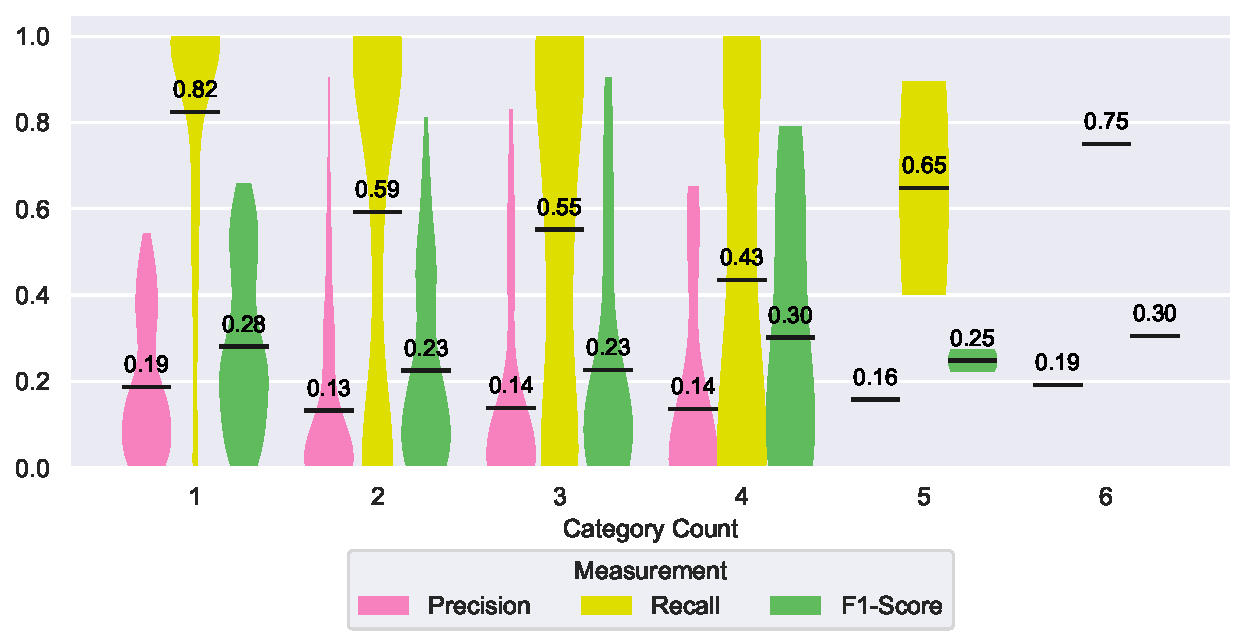
\includegraphics[width=\columnwidth,
		clip]{img/big-study/recall-precision-categorycount-KWS.pdf}
		\caption{structural category count
		in training and test sets.}
		\label{fig:recall-precision-categorycount-KWS}
\end{subfigure}
\caption{Precision, recall, and F$_{1}$-score of chunk retrieval with
Keyword Search (KWS) compared by \ldots}
\label{fig:results-KWS}
\end{figure*}


We present the precision,
recall, and F$_{1}$-score of the chunk retrieval runs with KWS in
\Cref{fig:results-KWS}.
Violin plots show the distribution the values of each measurement,
while the black horizontal lines show their average.
If the figure shows no violin plot for a measurement, we only have one
data point available or all values are the same.

\Cref{fig:recall-precision-examplecount-KWS} presents these
measurements for different
numbers of training examples.
The recall increases by about 12\% when
increasing the size of the training set to more than one example,
while the precision stays constant around 16\%.
The F$_{1}$-score
stays around 26\%.

\Cref{fig:recall-precision-categorycount-KWS} shows the same
measurements for an increasing number of structural categories in the
training and test examples.
For more than one structural category in
the training and test examples the recall decreases by about 20\% and
the precision decreases about 6\%.
For more than two structural
categories there is no clear trend in precision, recall, or
F$_{1}$-score.

% M: Perhaps, above in our section about logchunks, we would need some
% basic empirical stats -- e.g., how long are the files and how much
% do we usually extract from the log
% C: yup, that would be nice
% sadly, it's quite a bit of work to get those :/
% maybe I/We'll do it at the end
\subsubsection{Random Line Retrieval (RLR)}
\label{sec:r:rlr}
The baseline of randomly
picking lines from build logs delivers the expected low and
``random'' results: precision ranges between 5\% and 8\%,
recall between 6\% and 8\%.
As expected, the size of the training set has no impact on precision
or recall of retrieving chunks with RLR.
With a larger number of structural categories within the training and
test sets, the precision of RLR decreases from 7\% to 0\%, while
the recall varies between 0\% and 11\%.

\subsubsection{Comparison of All Techniques}
In this section, we compare the results of all four chunk retrieval
techniques and show the impact of structural categories on precision,
recall and F$_{1}$-scores of the different techniques.

% absolute results? is there a nice word for these results
\Cref{fig:success-partial-all} compares the results all of chunk
retrievals techniques in our study.
It shows how many runs per technique were successful, partially
successful or unsuccessful in retrieving the chunk defined in the
test example.
CTS and KWS
extract at least some of the desired lines in 79\% and 88.5\%
of the chunk retrieval runs.
With 38.25\%, KWS also has the highest proportion of fully
successful extractions, followed by PBE with 34.5\%.
PBE has the
lowest number of partial retrievals with only 18 out of 400 chunk
retrieval runs.
All techniques clearly outperform the random baseline (RLR).

\Cref{fig:category-all}
shows the influence of all training and test examples being from the
same structural category
(\Cref{fig:recall-precision-singlecategory-all})
compared to being from multiple categories
(\Cref{fig:recall-precision-multicategory-all}).
For more
than one category present, the recall of PBE decreases greatly.
For CTS and KWS the values also decrease, while RLR is not affected by
the number of structural categories present.
Again, all techniques---except for PBE with multiple structural
categories---yield better retrievals than RLR.

\begin{figure}[!t]
		\centering
		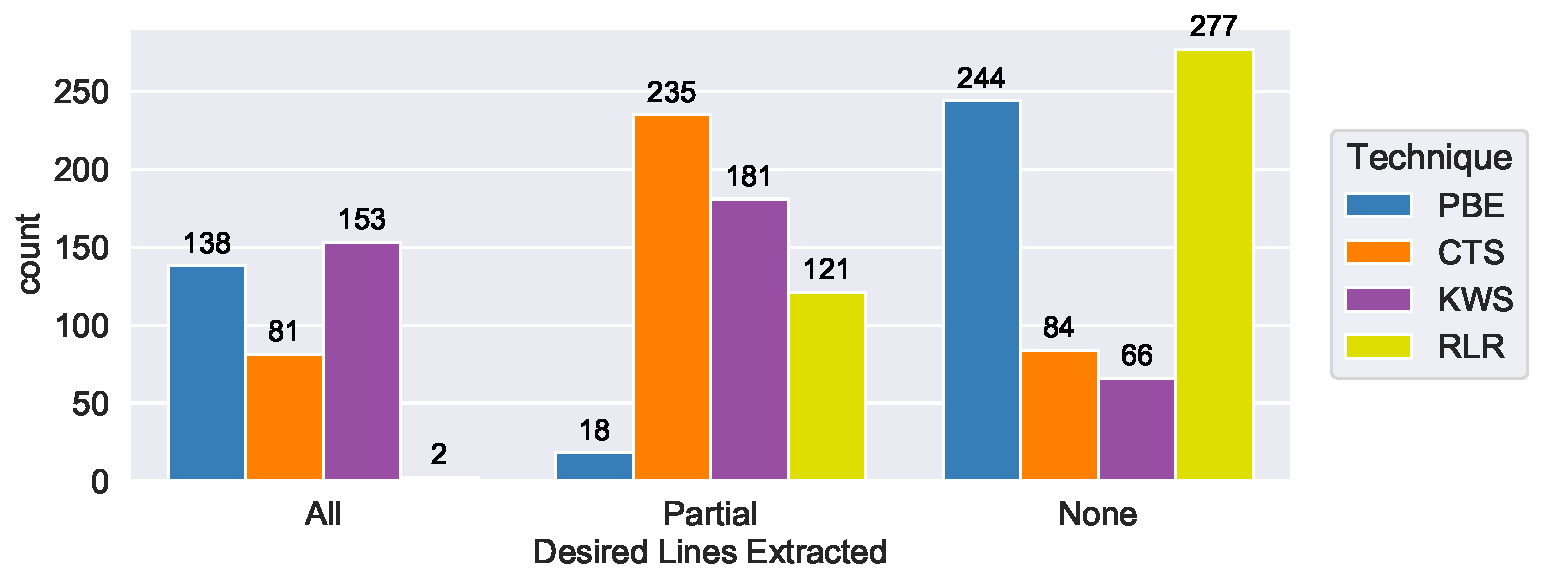
\includegraphics[width=\columnwidth,
		clip]{img/big-study/success-partial-all.pdf}
		\caption{Success of chunk retrievals across all
		techniques.}
		\label{fig:success-partial-all}
\end{figure}

\begin{figure*}
\centering
    \textbf{PBE, CTS, KWS, and RLR}\par\medskip
\begin{subfigure}[b]{\columnwidth}
		\centering
				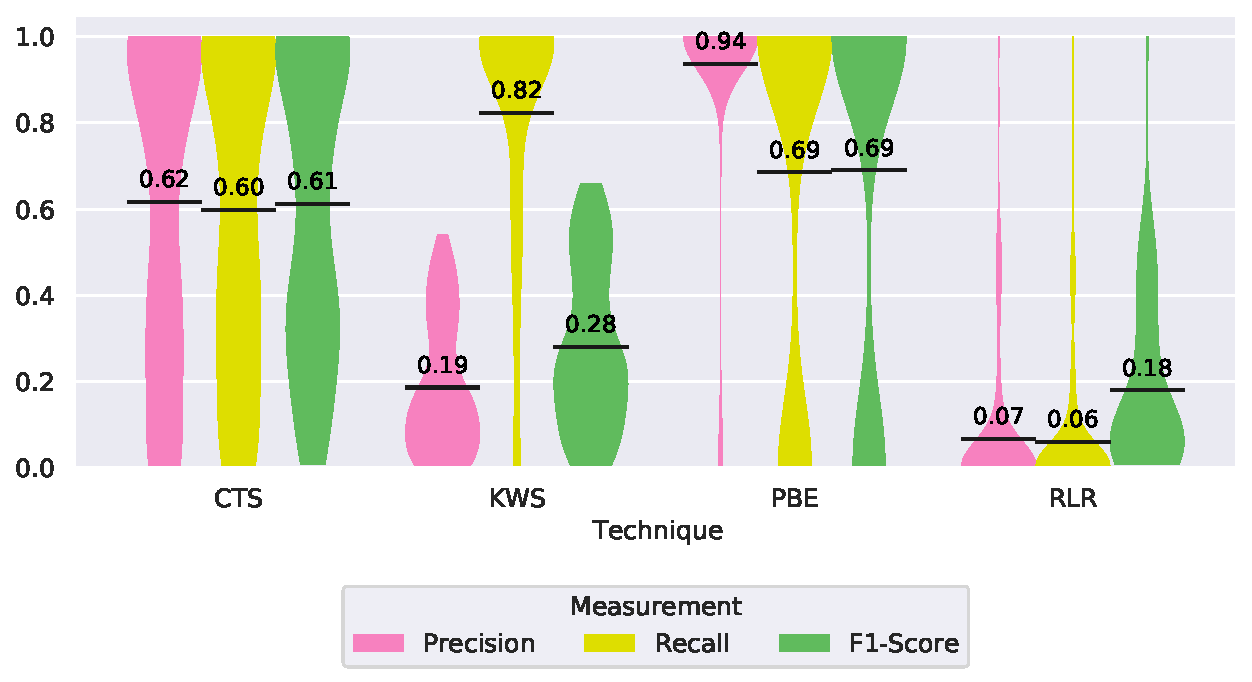
\includegraphics[width=\columnwidth,
				clip]{img/big-study/recall-precision-singlecategory-all.pdf}
		\caption{Training and test examples in 1
		structural category.}
		\label{fig:recall-precision-singlecategory-all}
\end{subfigure}\hspace{\fill}
\begin{subfigure}[b]{\columnwidth}
		\centering
				\centering
		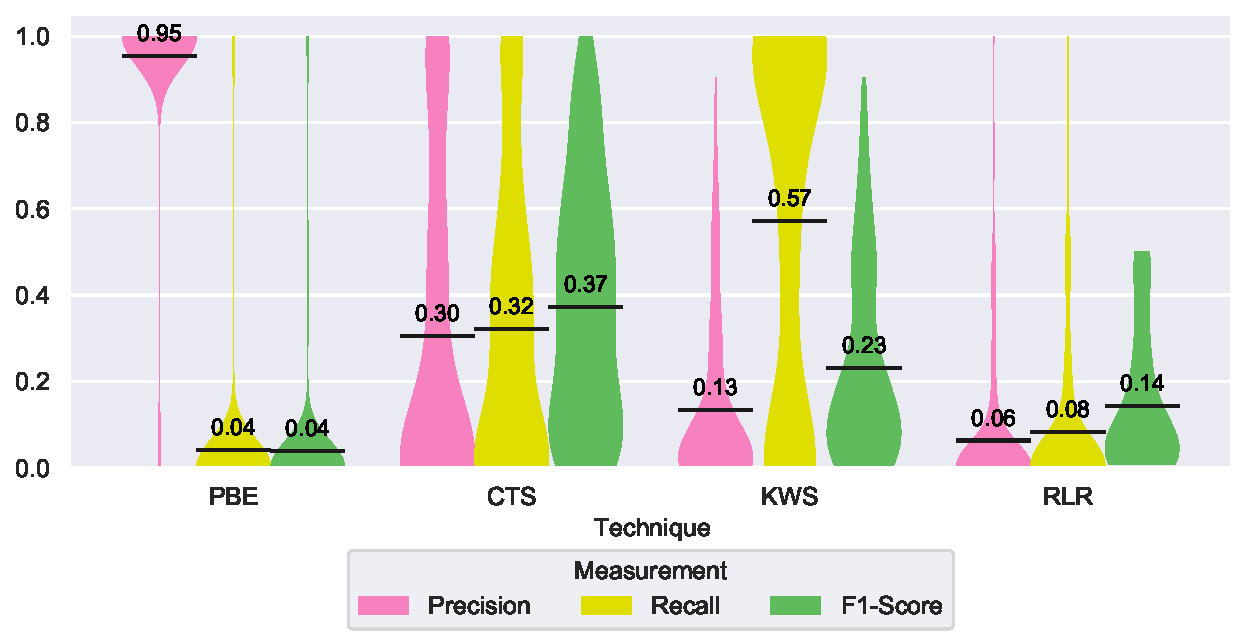
\includegraphics[width=\columnwidth,
		clip]{img/big-study/recall-precision-multicategory-all.pdf}
		\caption{Training and test examples in \textgreater
		1 structural
		category.}
		\label{fig:recall-precision-multicategory-all}
\end{subfigure}
\caption{Precision, recall, and F$_{1}$-score of all
techniques compared, split by structural category count.}
\label{fig:category-all}
\end{figure*}

\section{Discussion}
\label{sec:discussion}

For the interpretation of the study results, we look at each chunk
retrieval technique separately.
Next, we discuss
which criteria should influence the decision to use a certain
chunk retrieval technique most.
Based on the empirical comparison, we present a
decision tree between the three techniques we investigated.

\subsection{Interpretation of Study Results}
Following from the results of the empirical study,
we give recommendations for
which types of log chunks and how many training examples
each technique is suited, as well as
how their output can be used further.
We summarize these recommendations in
\Cref{tab:single-technique-recommendations}.

\begin{table}[tbp]
\caption{Recommendations for each of the investigated chunk retrieval
techniques.}
\label{tab:single-technique-recommendations}

\resizebox{\columnwidth}{!}{%
\centering
\begin{tabular}{llll}
  \toprule
  & \textbf{PBE} & \textbf{CTS} & \textbf{KWS} \\
  \midrule
  \textbf{Structural Categories} & 1 & less is better & \makecell[l]{best
  1 \\
  multiple okay} \\
  \midrule
  \textbf{Training Set Size} & 2 & no influence & 2 \\
    \midrule
  \textbf{Precision} & \makecell[l]{high \\ (if synthesis succeeds)} &
  medium &
  low \\
    \midrule
  \textbf{Recall} & \makecell[l]{high \\ (if synthesis succeeds)} &
  medium &
  high \\
    \midrule
  \makecell[l]{\textbf{Confidence in} \\ \textbf{Output Correctness}}
  & high & low &
  \makecell[l]{low (precision) \\ high (recall)} \\	\midrule
  \textbf{Output Consumer} & program & human & human \\
  \bottomrule
\end{tabular}%
}
\end{table}

\subsubsection{Program Synthesis by Example (PBE)}

\noindent
\textbf{Configuration and Input.}
The study results show that chunk retrieval with PBE gives best
results when the log chunks are structurally identical.
This is
because PROSE has difficulty synthesizing OR-based
programs~\cite{mayer2015user}.
PBE is thus suited to retrieve information
chunks that always have the same defining surrounding or internal
structure.
To extract for example the reason a build failed, the log
passage describing the failure would always have to start and
end the same way.

When the training examples are of the same structure, one or two
two training examples are enough input for PROSE to synthesize a regular
expression program with good recall.
In the study, additional training
examples from the same structural category
did not improve the chunk retrieval.
In fact, unless they
were in some sense redundant, adding more training examples even
hindered the applicability of PBE.

\noindent
\textbf{Retrieval Output Usage.}
If the program synthesis succeeds and applying the regular expression
program yields an output, PBE has high precision and recall.
The technique
clearly identifies a failing synthesis or when the regular expression
finds no match on a build log.
Therefore, if PBE produces
an output, the user can have high confidence that it is the desired
output.
This preciseness makes output from PBE chunk retrieval
well-suited for machine consumption and therefore automatic onward
processing.

\subsubsection{Common Text Similarity (CTS)}
\noindent
\textbf{Configuration and Input.}
Similar to PBE, chunk retrieval using CTS yields better results the
fewer structural categories are present in the training and test
examples.

The number of training examples had no noticeable influence on
precision or recall.
Information retrieval techniques
like text similarity commonly learn on a higher number of examples
than we chose in the study.
Future work should investigate how many
examples yield improvements in the chunk retrieval over a single
training example.

\noindent
\textbf{Retrieval Output Usage.}
CTS has good precision and recall on average, though with a high
variation.
This means that the quality of an output by CTS is hard to
determine, which makes it unsuited for automatic processing and requires
a human to further inspect and interpret the output.
This could include semi-automated procedures such as sending
developers an email with the extracted build failure reason.

\subsubsection{Keyword Search (KWS)}
\noindent
\textbf{Configuration and Input.}
KWS has a higher recall than the two other techniques for multiple
structural categories present in the training and test examples.
This
makes KWS a good technique if there is little prior knowledge of how
the targeted log chunk is represented in the build log.
For the
example of extracting the reason the build failed, KWS is best suited
if a build can fail in various steps logged by different build
tools and no
pre-categorization of where the build failed is available.

Going from one to two training examples, KWS's recall improves
significantly.
However, further enlarging the training set
does not lead to further improvements.

\noindent
\textbf{Retrieval Output Usage.}
While KWS has the highest recall of all three techniques, its
precision is the lowest.
The output of a chunk retrieval with KWS is
well-suited to be read by humans, but ill-suited for consumption by
automated tools.


\subsection{Recommendation of Suitable Techniques}

\begin{figure}[bt]
		\centering
		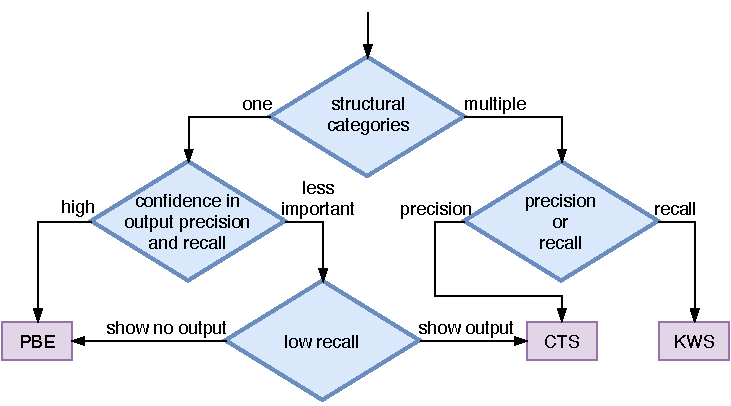
\includegraphics[width=\columnwidth,
		clip]{img/crt-recommendation.pdf}
		\caption{Decision tree for chunk
		retrieval techniques.}
		\label{fig:crt-recommendation}
\end{figure}

We saw that each of the techniques is suited for different types of
log chunks and the output of each is suited for different uses.
Now, we unify these results into conditions to answer
our second research question;
If researchers or developers want to retrieve chunks from build logs,
they can follow these conditions to identify the technique
suited best for their use case.
% I want to ref the figure early bc I believe the text is easier
% to follow when looking at the figure as well
We summarize these conditions in the decision tree in
\Cref{fig:crt-recommendation}.
It is built up of questions
which either lead to more questions or to a leaf node containing a
recommended technique.
In the next section we give two concrete examples on how to
apply our decision tree.


% we can't just have a paragraph in a scientific paper start with
% Caveat, I think ;-) Also, we should say why we THINK this is not
%the case.
% Otherwise we weaken our work unduly
% Of course we can! xD
% Agree with the rest.
% It's in TtV, quite close actually
% so I'll comment this out
% also #more selling :D
% \textbf{Caveat!}
% This is a preliminary hypothesis based on the results
% from our comparison study.
% The recommendations could therefore be
% influenced by idiosyncrasies of our specific implementation of the
% chunk retrieval techniques as well as the \emph{LogChunks}
% data set.

The first and most important aspect that influences a choice for
a chunk retrieval technique are the structural categories.
In other words:
are the targeted log chunks always presented in
the same structural way within the build logs?
Then the
chunks in all training examples and the analyzed build log are in the
same structural category.
This is why the first question in \Cref{fig:crt-recommendation} asks
how many structural categories the targeted log chunks have.

If the chunks are from multiple structural categories
and recall is more important than precision we recommend
to use KWS\@.
If precision is more important than recall, we
recommend CTS, as \Cref{fig:crt-recommendation} shows on the
right half of the decision tree.
We also recommend CTS when the log chunks are
from one structural category, when the user does not require high
confidence in the precision or recall of the outcome and when one
would rather have output with low recall instead of no output at all.
On the leftmost path of the decision tree,
when the chunks are from one structural category and the user
wishes high confidence in the correctness of the output or prefers
no output over output with low recall, we recommend PBE\@.

As a final recommendation, one could create a ``super analyzer'' by
combining the different build log analysis techniques studied in this
paper.
Such a super analyzer would likely always first employ PBE
(because of its high accuracy), followed by a combination of CTS and
KWS\@.
Other than initial setup and training time, there is no
downside to this approach if it is implemented in a transparent way to
the underlying technique: the output of the super analyzer could
include from which sub-technique it originated and thus facilitate
automatic onward processing or interpretation of the result.


\subsection{Exemplary Recommendation}
To illustrate how one would use the decision tree to find a suitable
chunk retrieval technique we describe two concrete examples: a software
team
wanting to monitor their build performance and a
researcher investigating why builds fail.

In the first example, a software development team wants to monitor
the performance of the phases within their CI build.
They are using
Travis CI, which measures the duration of build phases and documents
this within the build log.
As all log statements that report timing
measurements are formatted the same way, the targeted log chunks are
from one structural category.
Therefore, following the leftmost path in
\Cref{fig:crt-recommendation},
the development team should use
PBE to retrieve the duration of a build phase.

In the second example, a researcher wants to investigate whether
small or large groups of test cases
cause CI build failures.
They gather
CI build logs from various projects.
The task of the researcher is to extract the names of the
failing test cases from each build log.
When they use the
decision tree to select a chunk retrieval technique, they
first have to estimate how uniform the representation of the failing
test cases is in the investigated build logs.
As the researcher is
covering a wide range of test tools, the
log chunks they target are in various, non-predictable structural
representations.
The next question is whether they value precision
over recall.
As they have to manually inspect the results of both CTS
and KWS, they choose recall over precision to avoid having to inspect
the whole log in case the relevant chunk---the name of the failing
test case---was not retrieved.
Therefore, following the rightmost path in
\Cref{fig:crt-recommendation},
the decision tree recommends the researcher to use KWS\@.

In case the researcher wants to avoid manually inspecting the
retrieval results, they have to first separate the CI build logs
according to the test tool responsible for logging the test results.
Then the targeted log chunks are from one structural category and they
can use PBE, trained with examples from each test tool separately.

\section{Threats to Validity}
There are several threats to the validity of the conclusions of our
work.

\textbf{Implementation.}
Our results depend on the implementation of the investigated chunk
retrieval techniques and the libraries we used.
The program synthesis provided by PROSE is the basis for our
implementation of PBE\@.
The
idiosyncrasies of this framework influence the PBE results.
Other
frameworks similar to PROSE might have somewhat different strengths
and weaknesses.
For example, the need for examples from a single
structural category stems from the fact that PROSE cannot learn
regular expression programs with arbitrary boolean conjunctions and
disjunctions~\cite{mayer2015user}.
PROSE introduced this constraint to
keep the synthesis performance reasonable.
At the same time, this is
clearly a current theoretical challenge of all PBE implementations,
and we therefore attribute it to the technique itself, rather than the
specific implementation.

The library
{\tt text2vec}~\cite{text2vec2019webpage}
and the way it splits strings into word tokens is influencing
our implementation of CTS\@.
On the other hand,
{\tt text2vec} is the de-facto standard library to do word embeddings
in R.
We intentionally chose a simple, minimally configured or tuned
approach to compare against.
Tuning the text similarity
meta-parameters more to the specific use case of chunk retrieval from
build logs would yield better chunk retrieval results.

% kinda uncreative..
% not sure what another example would be?
% not sure if this adds much on top of the sentences further up
Overall, we believe our implementations and their weaknesses stand
prototypical for the techniques.
We tried to limit idiosyncrasies as much as possible, by choosing
standard approaches and configurations.

\textbf{Data Set.}
The build logs from the \emph{LogChunks} data set highly affect
the outcomes of the comparison study.
\emph{LogChunks} consists of build
logs from open source projects and therefore it is not clear whether
our results apply to industry projects that use build tools
not popular in open source development.
However, since \emph{LogChunks} covers a wide array of build tools and
programming languages,
we believe that the findings do generalize.
We collected build logs from Travis CI.
Yet, the format of the log chunk we chose
for the evaluation is largely independent of Travis CI\@.
This
is because the reason the build failed is described within the build
logs by the tools themselves and not the Travis CI environment.

\textbf{Training Set Size.}
Especially the results for CTS might be influenced by the fact that we
only trained on one to five examples.
We chose this small training set
size as a user has to provide the training examples
per project and one of the central aims of the chunk
retrieval techniques is that they can be set up wit little effort.
The fact that PBE and KWS performed best with already two training
examples shows that the training set size is large enough to
compare the three techniques.

\textbf{Few Samples with Many Structural Categories.}
Our comparison study shows fewer measurements with many structural
categories than with one structural category category (50.25\% one,
33.75\% two, 13.75\% more than two).
This stems from the fact that we
investigated the chunk retrieval techniques on a real-world data set,
where there were mostly few structural categories within one project.
In addition, the third of the measurements we conducted with two
structural categories already showed the negative effect of an
increasing number of structural categories on the performance of the
chunk retrieval techniques.

\section{Future Work}
% Actually, this future work is very, *very* good.
%It might be
% the best future work I have ever read in an article.
% One idea would be to sell it as such and tie a bit back to our
% first literature survey.
%You can say you give a roadmap to guide
% future research in the field, and sell it in abstract and intro!

There are various future research opportunities based on the
work we presented:

\textbf{Systematic Survey of Industry Approaches for Build
Log Analysis.}
Our survey is limited to academic work and articles.
However, handling build logs is a challenge for a wide range of
practitioners as well.
We propose to investigate the techniques used in industry to analyze
build logs.
An example is the Jenkins \emph{build-failure-analyzer}
plugin~\cite{jenkins2020failure-analyzer} or automatically
inferred test results in Azure~\cite{azure2020inferred}.

\textbf{Further Analysis of \emph{LogChunks}.}
We created the
\emph{LogChunks} data set \cite{brandt2020logchunks} specifically for
the comparative
study in this paper, though it can be the basis for various further
analyses of build log data.
The keywords, for example, can be
investigated to answer which keywords are used to search for the
reason the build failed within build logs.

\textbf{Cross-Project Build Log Analysis.}
We trained and
tested each chunk retrieval technique on examples from the same
project.
We propose to analyze how techniques could be trained
across projects, building the cornerstones for build
environment-agnostic analysis tools.
This has the advantage of creating
a default build log analyzer that would work without any pre-training.

\textbf{Comparison with more Chunk Retrieval Techniques.}
This
paper investigates the three chunk retrieval techniques PBE, CTS, and
KWS\@.
Our study design can be reused to evaluate other build log
analysis techniques, such as the parser Tomassi et al.
used to create
BugSwarm~\cite{tomassi2019bugswarm} or the regex-based approach
Beller et al.
used to create TravisTorrent~\cite{beller2017oops}.

\textbf{Refinement of Retrieval Quality for each Technique.} We
investigated basic configurations of existing techniques applied to
chunk retrieval from build logs.
In a next step, each of these
techniques could be refined to better approach the domain of build
logs.
The \emph{LogChunks} data set and our study results act as a
baseline to benchmark such technique improvements.
We propose the
following improvements:
\begin{itemize}[leftmargin=0.4cm]
  \item \textbf{Custom Ranking and Tokens for PBE.} The program
  synthesis through PROSE ranks possible programs according to
  what the user most likely intended.
  One could adapt the ranking
  rules provided by the FlashExtract DSL to fit common build log
  chunk retrieval tasks.
  FlashExtract includes special tokens when
  enumerating possible regular expressions.
  One could extend these
  with tokens found in build logs, such as ``-,''
	``=,'' ``ERROR,''
  or ``[OK]''.
  \item \textbf{Meta-Parameter Optimization for CTS.} Information
  retrieval techniques have various meta-parameters which can be
  optimized for the specific use
  case~\cite{panichella2016parameterizing}.
  We propose to further
  investigate improvements in preprocessing of the log text, in
  tokenization of the log lines into terms and in stop words
  lists.
\end{itemize}

\textbf{Usability Analysis of Chunk Retrieval Output.}
Our
analysis of the chunk retrieval output focuses on
precision and recall.
A next step could be to investigate how useful these
outputs really are to developers through controlled experiments or
user studies.

\section{Conclusion}
\label{sec:conclusion-fw}

The goal of this paper is to support practitioners and researchers in
their decision on how to analyze build logs.
To this end, we
conducted a systematic mapping survey to map out the available build
log analysis techniques.
We saw that, while build log analysis is widely used, it is often
a side part of a work and implementations are rarely reused.
This shows the need for a new generation of generic and automated
build log analysis techniques that need little effort to set up.

Based on common approaches we observed in literature,
we implemented three promising chunk retrieval techniques:
PBE synthesizes regular expression programs based on examples of logs
and corresponding chunks, CTS leverages a common text similarity
measure to retrieve those lines which are most similar to example
chunks, and KWS finds the targeted chunks in a build log by searching
for identifying keywords.

We evaluated the performance of these chunk retrieval techniques on the
\emph{LogChunks} data set and saw varying results.
CTS had the highest average F$_{1}$-score with 51\%, while the other
techniques showed higher average scores for precision (95\%, PBE)
and recall (70\%, KWS).

To guide researchers and developers on which technique suits their
use case,
we summarized our results in a decision tree.
We found
that the structural representation of the targeted information in the
build logs is the main factor a user should consider when they
choose a
technique.
Secondary factors are the desired confidence in recall and
precision of the produced output and whether precision or recall is
more important for the task at hand.

Finally, we gave an
outline to guide future research efforts in the area of build log
analysis.
Important themes are a systematic investigation of industry approaches,
benchmarks of existing build log analysis approaches and further
refinement of the chunk retrieval techniques we proposed.
We strongly believe that further research into the techniques to
analyze build logs will support researchers and developers alike to
leverage the vast amounts of valuable information
hidden within build logs.
